% Chapter 1

\chapter{Background and work related to the M/EEG inverse problem} % Main chapter title
\label{chapter:background} % For referencing the chapter elsewhere, use \ref{Chapter1} 
\noindent\makebox[\linewidth]{\rule{0.75\paperwidth}{0.4pt}}
\noindent\makebox[\linewidth]{\rule{0.75\paperwidth}{0.4pt}}

\localtableofcontents % local toc

\noindent\makebox[\linewidth]{\rule{0.75\paperwidth}{0.4pt}}
\noindent\makebox[\linewidth]{\rule{0.75\paperwidth}{0.4pt}}

\newpage
%----------------------------------------------------------------------------------------

% Define some commands to keep the formatting separated from the content 
\newcommand{\keyword}[1]{\textbf{#1}}
\newcommand{\tabhead}[1]{\textbf{#1}}
\newcommand{\code}[1]{\texttt{#1}}
\newcommand{\file}[1]{\texttt{\bfseries#1}}
\newcommand{\option}[1]{\texttt{\itshape#1}}


%--------- Signal sources of MEEG recording-----------------------------------------------
\section{Signal sources of MEG and EEG recordings}
%Measuring weak MEG/EEG signals in the background of strong environmental noise, having a noise level of several orders of magnitude larger than the MEG/EEG signals, is a challenging task. 
At the cellular level of the brain, its nervous system is defined by the presence of a special type of neural cells. Despite the apparent simplicity in the structure of the neural cell, the biophysics of the neural current flow relies on a complex network of billions of cells, neurons and glial cells~\cite{baillet2001electromagnetic, hodgkin1964conduction}. Neurons are nerve cells that transmit nerve signals to and from the brain. They are about 100 billions neurons. The neuron consists of a cell body (or soma) with branching dentrites (signal receivers). They send these signals in the form of electrochemical waves traveling along thin fibers called axons, which cause chemicals called neurotransmitters to be released at junctions called synapses. A cell that receives a synaptic signal from a neuron may be excited, inhibited, or otherwise modulated. At a synapse, the cell that sends signals is called presynaptic, and the cell that receives signals is called postsynaptic.\\

Every neuron maintains a voltage gradient across its membrane, due to metabolically driven differences in ions of sodium, potassium, chloride and calcium within the cell, each of which has a different charge. If the voltage changes significantly, an electro-chemical pulse called an action potential (or nerve impulse) is generated. This electrical activity can be measured and displayed as a waveform called brain wave or brain rhythm. This pulse travels rapidly along the cell's axon, and is transferred across a synapse to a neighbouring neuron, which receives it through its feathery dendrites. Each individual neuron can form thousands of links with other neurons in this way, giving a typical brain well over 100 trillion synapses (up to 1,000 trillion, by some estimates).\\

Roughly, when a neuron is excited by other —and possibly remotely located— neurons via an afferent volley of action potentials, \ac{EPSP}s are generated at its apical dendritic tree. The apical dendritic membrane becomes transiently depolarized and consequently extracellularly electronegative with respect to the cell soma and the basal dendrites. This potential difference causes a current to flow through the volume conductor from the nonexcited membrane of the soma and basal dendrites to the apical dendritic tree sustaining the EPSPs~\cite{gloor1985neuronal}.
Some of the current takes the shortest route between the source and the sink by traveling within the dendritic trunk. Conservation of electric charges imposes that the current loop be closed with extracellular currents flowing even through the most distant part of the volume conductor. Intracellular currents are commonly called primary currents, while extracellular currents are known as secondary, return, or volume currents.\\

Both primary and secondary currents contribute to magnetic fields outside the head and to electric scalp potentials, but spatially structured arrangements of cells are of crucial importance to the superposition of neural currents such that they produce measurable fields. Tens of thousands of synchronously activated large pyramidal cortical neurons are thus believed to be the main MEG and EEG generators because of the coherent distribution of their large dendritic trunks locally oriented in parallel, and pointing perpendicularly to the cortical surface~\cite{nunez2000relationship}. The currents associated with the EPSPs generated among their dendrites are believed to be at the source of most of the signals detected in MEG and EEG because they typically last longer than the rapidly firing action potentials traveling along the axons of excited neurons~\cite{nunez2006electric}. %Indeed, calculations such as those shown in~\cite{hamalainen1993magnetoencephalography} suggest each synapse along a dendrite may contribute as little as a 20 fA-m current source, probably too small to measure in MEG/EEG. Empirical observations instead suggest we are seeing sources on the order of 10 nA-m, and hence the cumulative summation of millions of synaptic junctions in a relatively small region. Nominal calculations of neuronal density and cortical thickness suggest that the cortex has a macro-cellular current density on the order of 100 nA/mm2.\\

\begin{figure}
	\centering
	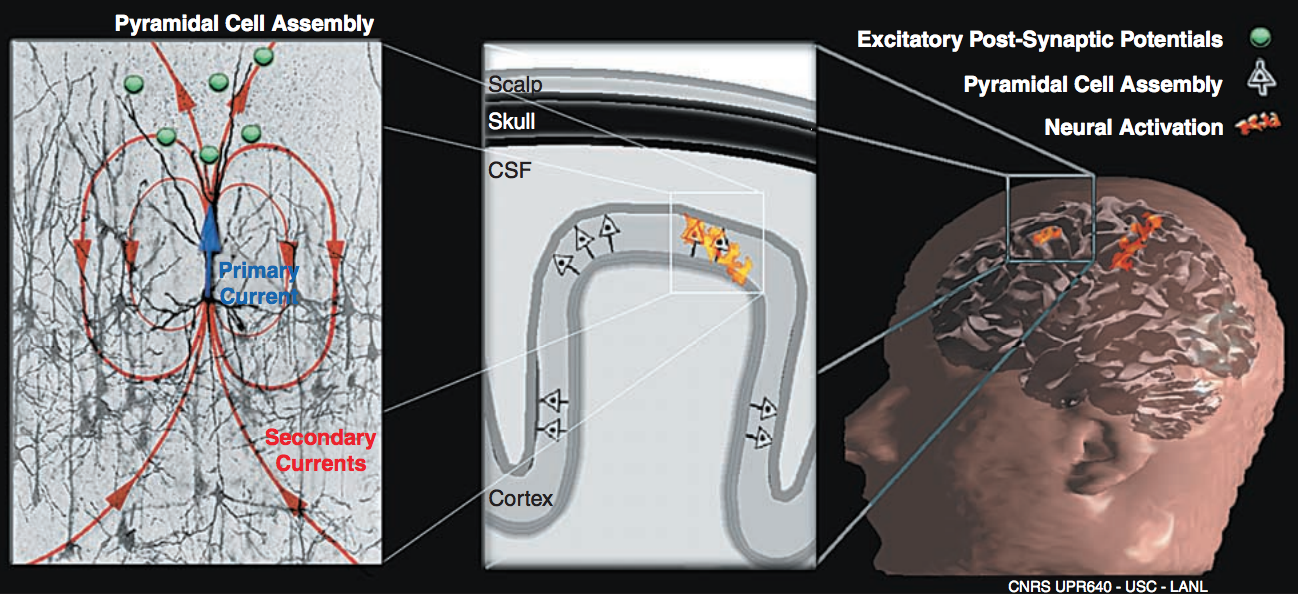
\includegraphics[width=0.95\textwidth]{background/network_cortical_neural_cells}
    \caption{Networks of cortical neural cell assemblies are the main generators of MEG/EEG signals. Left: Excitatory postsynaptic potentials (EPSPs) are generated at the apical dendritic tree of a cortical pyramidal cell and trigger the generation of a current that flows through the volume conductor from the non-excited membrane of the soma and basal dendrites to the apical dendritic tree sustaining the EPSPs. Center:  Large cortical pyramidal nerve cells are organized in macro-assemblies with their dendrites normally oriented to the local cortical surface. This spatial arrangement
and the simultaneous activation of a large population of these cells contribute to the spatio-temporal superposition of the elemental activity of every cell, resulting in a current flow that generates detectable EEG and MEG signals. Right: Functional networks made of these cortical cell assemblies and distributed at possibly mutliple brain locations are thus the putative main generators of MEG and EEG signals. The origin of this image is~\cite{baillet2001electromagnetic}.
    }
    \label{fig:network_cortical_neural_cells}
\end{figure}

MEG and EEG are non-invasive functional imaging techniques for analyzing the neuronal activity on a macroscopic scale. In contrast to indirect neuroimaging modalities, MEG and EEG signals derive from the net effect of ionic currents flowing in the dendrites of neurons during synaptic transmission. In accordance with Maxwell's equations, any electrical current will produce a magnetic field, and it is this field that is measured. The measurement principle of MEG and EEG is illustrated in Figure~\ref{fig:meg_eeg_principle}.\\

The neuronal activity captured by MEG is not, as perhaps expected, generated by the (too brief) axonal action potentials of pyramidal cells, but rather by the net contributions of excitatory and inhibitory dendritic postsynaptic potentials. This current flow through the apical dendrites (represented as a ‘dipole’) generates a magnetic field that projects radially; thus, MEG excels at detecting dipoles arranged in a tangential orientation to the skull. Fortunately, the extensively folded sulci of the human cortex promote that orientation for the majority of cortical microcolumns. However, MEG is less sensitive to deeper (including subcortical) sources, as the magnetic field change decreases rapidly with distance.\\

\begin{figure}
	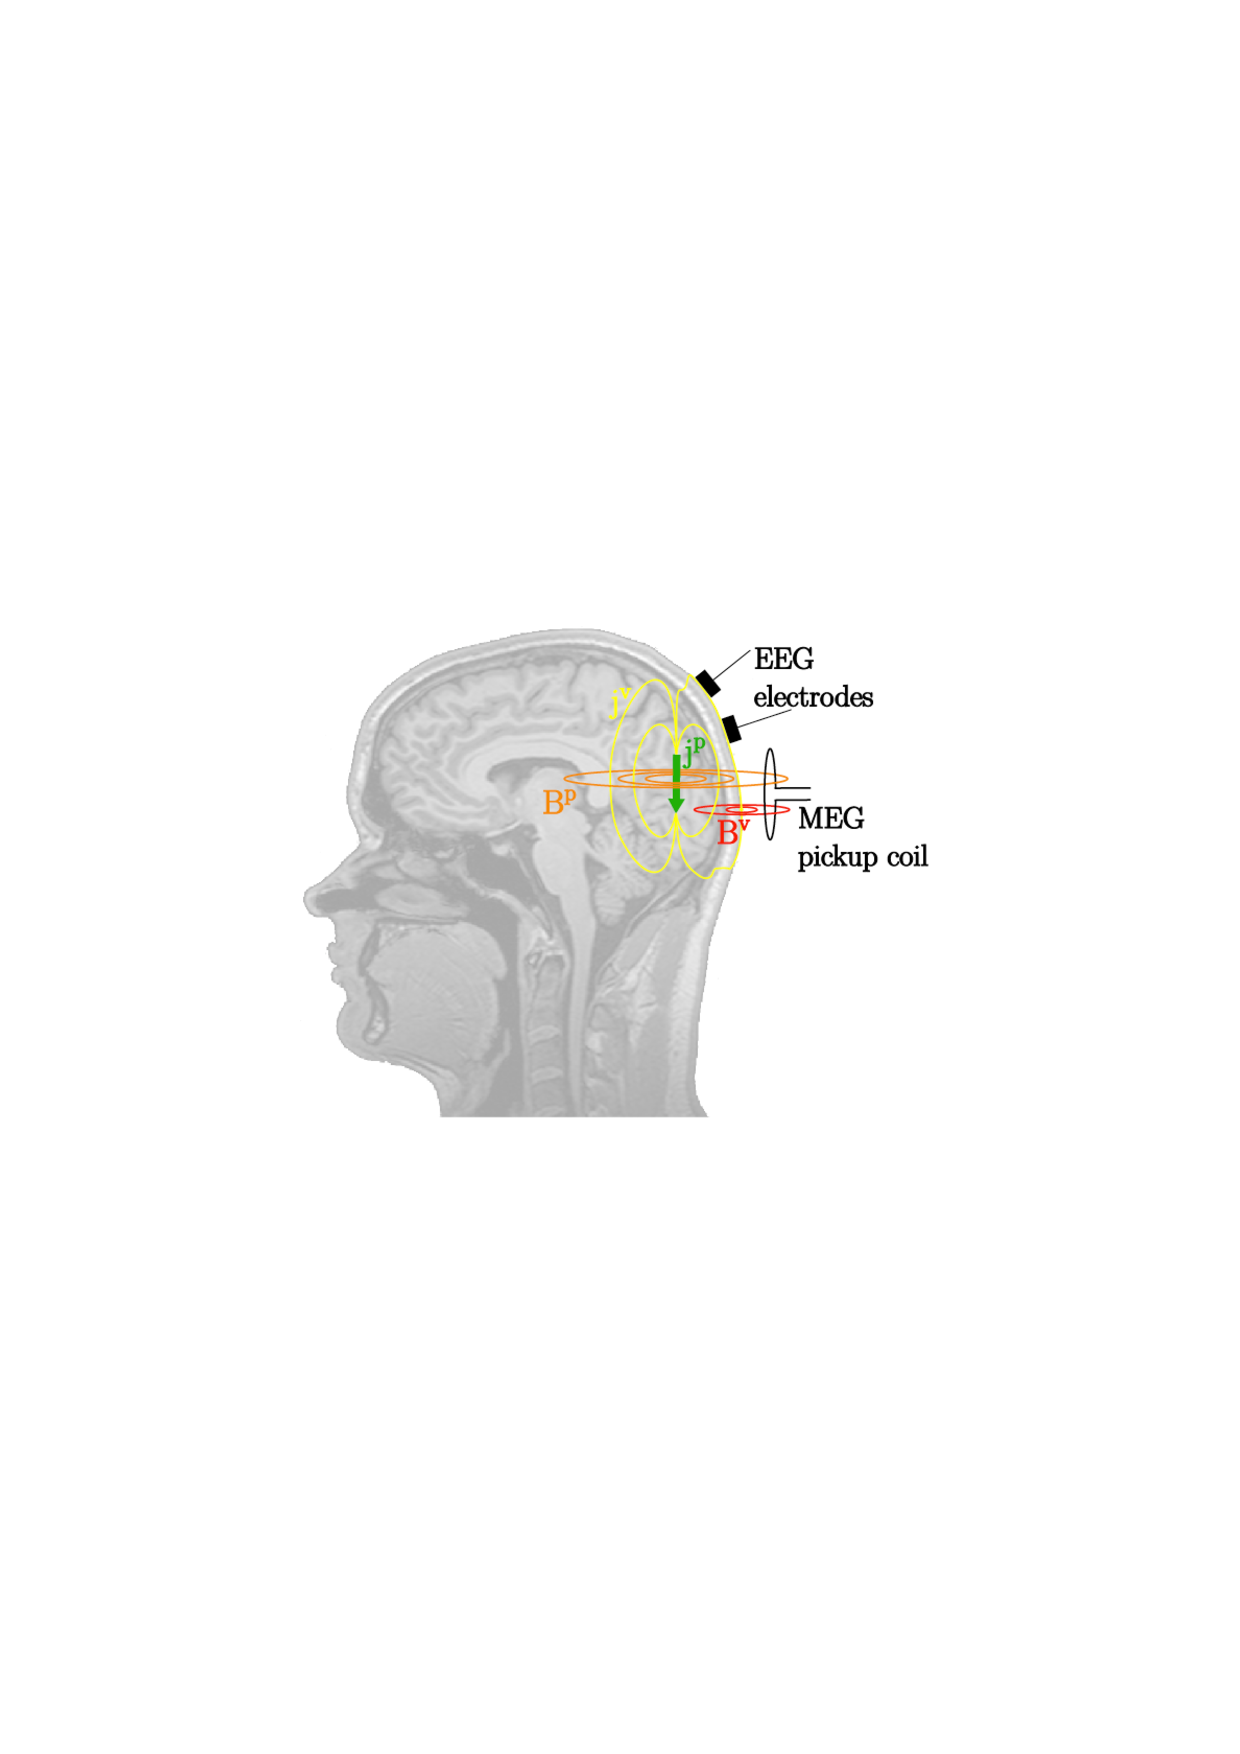
\includegraphics[trim={1cm 10cm 2cm 10cm},width=0.95\textwidth]{background/meg_eeg_principle}
    \caption{Simplified model of the measuring principle of MEG and EEG. The EEG measures the difference of the electric potential between the EEG electrode and a reference due to volume currents generated by primary currents in the brain. The
MEG captures the magnetic field generated by both primary and volume currents.
    }
    \label{fig:meg_eeg_principle}
\end{figure}

In 1969, the journey to understand the electrical potentials of the brain took an interesting and fruitful detour when David Cohen, a physicist working at MIT, became the first to confidently measure the incredibly tiny magnetic fields produced by the heart's electrical signals. To do this, he constructed a shielded room, blocking interference from the overwhelming magnetic fields generated by earth itself and by other electrical devices in the vicinity, effectively closing the door on a cacophony of voices to carefully listen to a slight whisper. His shielding technique became central to the advent of MEG, which measures the yet even quieter magnetic fields generated by the brain's electrical activity.\\ % XXX add ref

This approach to record the brain's magnetic fields, rather than the electrical potentials themselves, was advanced even further by James Zimmerman and others working at the Ford Motor Company, where they developed the SQUID, a Superconducting QUantum Interference Device. A SQUID is an extremely sensitive magnetometer, operating on the principles of quantum physics, which is able to detect precisely those very tiny magnetic fields produced by the brain. To appreciate the contributions of magnetic shielding and SQUIDs to magnetoencephalography, consider that the earth's magnetic field, the one acting on your compass needle, is at least 200 million times the strength of the fields generated by your brain trying to read that very same compass.\\

On the other hand, the EEG measures the electric potential difference between the EEG electrode and a reference on the scalp associated with primary currents in the brain. These electric potential differences, which are in the range of a few microvolts, are recorded using amplifiers with high open-loop gain, common-mode rejection ratio, and input impedance. The first human EEG recording was done by Hans Berger in 1924.\\

MEG and EEG can be recorded simultaneously and reveal complementary properties of the electrical fields. Although the signals of EEG and MEG are generated by the same sources (electrical currents in the brain), they are both sensitive to different aspects of these sources. This could be compared to viewing the shadows of the same object from two different angles; combining the two recordings usually leads to better source estimation~\cite{malmivuo2012comparison,sharon2007advantage,aydin2015combined}.

%--------- Forward model -------------------------------------------------------------------
\section{The forward model}
The bioelectromagnetic forward problem describes the relationship between a given neural activity in the brain and the observable MEG and EEG signals. We assume the electric current (denoted by $\vec{j}_t(\vec{r})$) at any position (denoted by $\vec{r}$ in the head is known at arbitrary time $t$. The magnetic field or the scalp voltage detected by one sensor can be modeled as an integration or a linearly weighted combination of the currents at all positions, using Maxwell's equations under a reasonable head model that describes the shape, the electrical conductivity and the permeability of various tissues~\cite{hamalainen1993magnetoencephalography,mosher1999eeg}.

\subsection*{Maxwell's equations}
We consider the head as a finite three-dimensional volume conductor, non magnetic. The quasi-static approximation of Maxwell's equations are a set of partial differential equations forming the foundation of classical electromagnetism. We denote by $\mathbf{E}$ the electric field, $\mathbf{B}$ the magnetic field, $\mathbf{J}$ the current density, and $\rho$ the charge density.

\begin{center}
$\left\{
\begin{array}{l}
  \nabla . \mathbf{E} = \frac{\rho}{\epsilon} \\
  \nabla \times \mathbf{E} = \frac{-\partial \mathbf{B}}{\partial t} \\
  \nabla \cdot \mathbf{B} = 0 \\
  \nabla \times \mathbf{B} = \mu_0 (\mathbf{J} + \epsilon\frac{\partial \mathbf{E}}{\partial t})
\end{array}
\right.$
\end{center}

For the biological signals of interest in MEG/EEG, the time-derivatives of the associated electric and magnetic fields are sufficiently small to be ignored in Maxwell’s equations. Recent discussions and details of this quasi-static approximation can be found in\cite{hamalainen1993magnetoencephalography,tripp1983physical,heller1992brain}.\\

The propagation of the electric potentials and magnetic field measured by EEG and MEG suffers from no temporal delay, meaning that the recording is instantaneous. Let us note $\mathbf{M}\in\RR^{N\times T}$ the measurement matrix of MEG/EEG, $\mathbf{G}\in\RR^{N\times SO}$ the design matrix (leadfield or gain matrix~\cite{h1994}) with $S$ source locations in the brain and $O$ number of orientations (1 or 3). One has:
\begin{equation}
\mathbf{M} = \mathbf{GX}+\mathbf{E}
\end{equation} \label{eq:meeg_ip}
\noindent From now on, $\mathbf{E}$ denotes an additive white Gaussian noise. Equation~\eqref{eq:meeg_ip} is linear not by assumption but by guarantee from Maxwell's equations.\\

If the source orientation is set a priori, \textit{e.g.}, by using the cortical constraint assuming sources to be oriented perpendicularly to the cortical surface~\cite{Dale:1993} (O = 1), a single dipole with unit norm per source location is used to compute the gain matrix $\mathbf{G}\in\RR^{S\times T}$. To allow for arbitrary dipole orientations, the dipole moment per location is represented by a linear combination of O perpendicular unit dipoles. An orthogonal dipole triplet is commonly applied (O = 3). Due to the low sensitivity of MEG to radial sources, the radial component per source location is sometimes neglected (O = 2). The gain matrix $\mathbf{G}$ is generated by solving the MEG/EEG forward problem for each dipole separately and by appending the results column-wise. Hence, each column of the gain matrix provides information on the topography in the sensor space generated by the activity of a specific unit dipole, while each row reflects the sensitivity of a specific sensor to all unit dipoles in the model.

\subsection*{Spherical head models}
A very common approximation in the forward modeling consists in assuming that the head is a set of nested concentric spheres, each corresponding to a layer with homogeneous and isotropic conductivity (Figure~\ref{fig:sphere_align}). Typically, the head is represented by three to five regions, \textit{e.g.}, scalp, skull, cerebrospinal fluid, gray matter, and white matter, and that the conductivity is constant and isotropic within these regions. The gradient of the conductivity is therefore zero except at the surfaces between regions. Computable analytic solutions exist for both MEG and EEG forward problems.\\

A very practical formulation of the EEG and MEG field kernels has been presented by Mosher~\cite{mosher1999eeg}, that only requires vectors expressed in their Cartesian form. For MEG, since the magnetic permeability does not change across layers (and does not change much from the vacuum) and no current exists outside the head (where the sensors are located), the full magnetic field outside a set of concentric spheres can be calculated without explicit consideration of the volume currents. Therefore, the MEG spherical model does not require specifying (or assuming) the number of and the radius ratios between the spherical layers.\\

\begin{figure}
\centering
	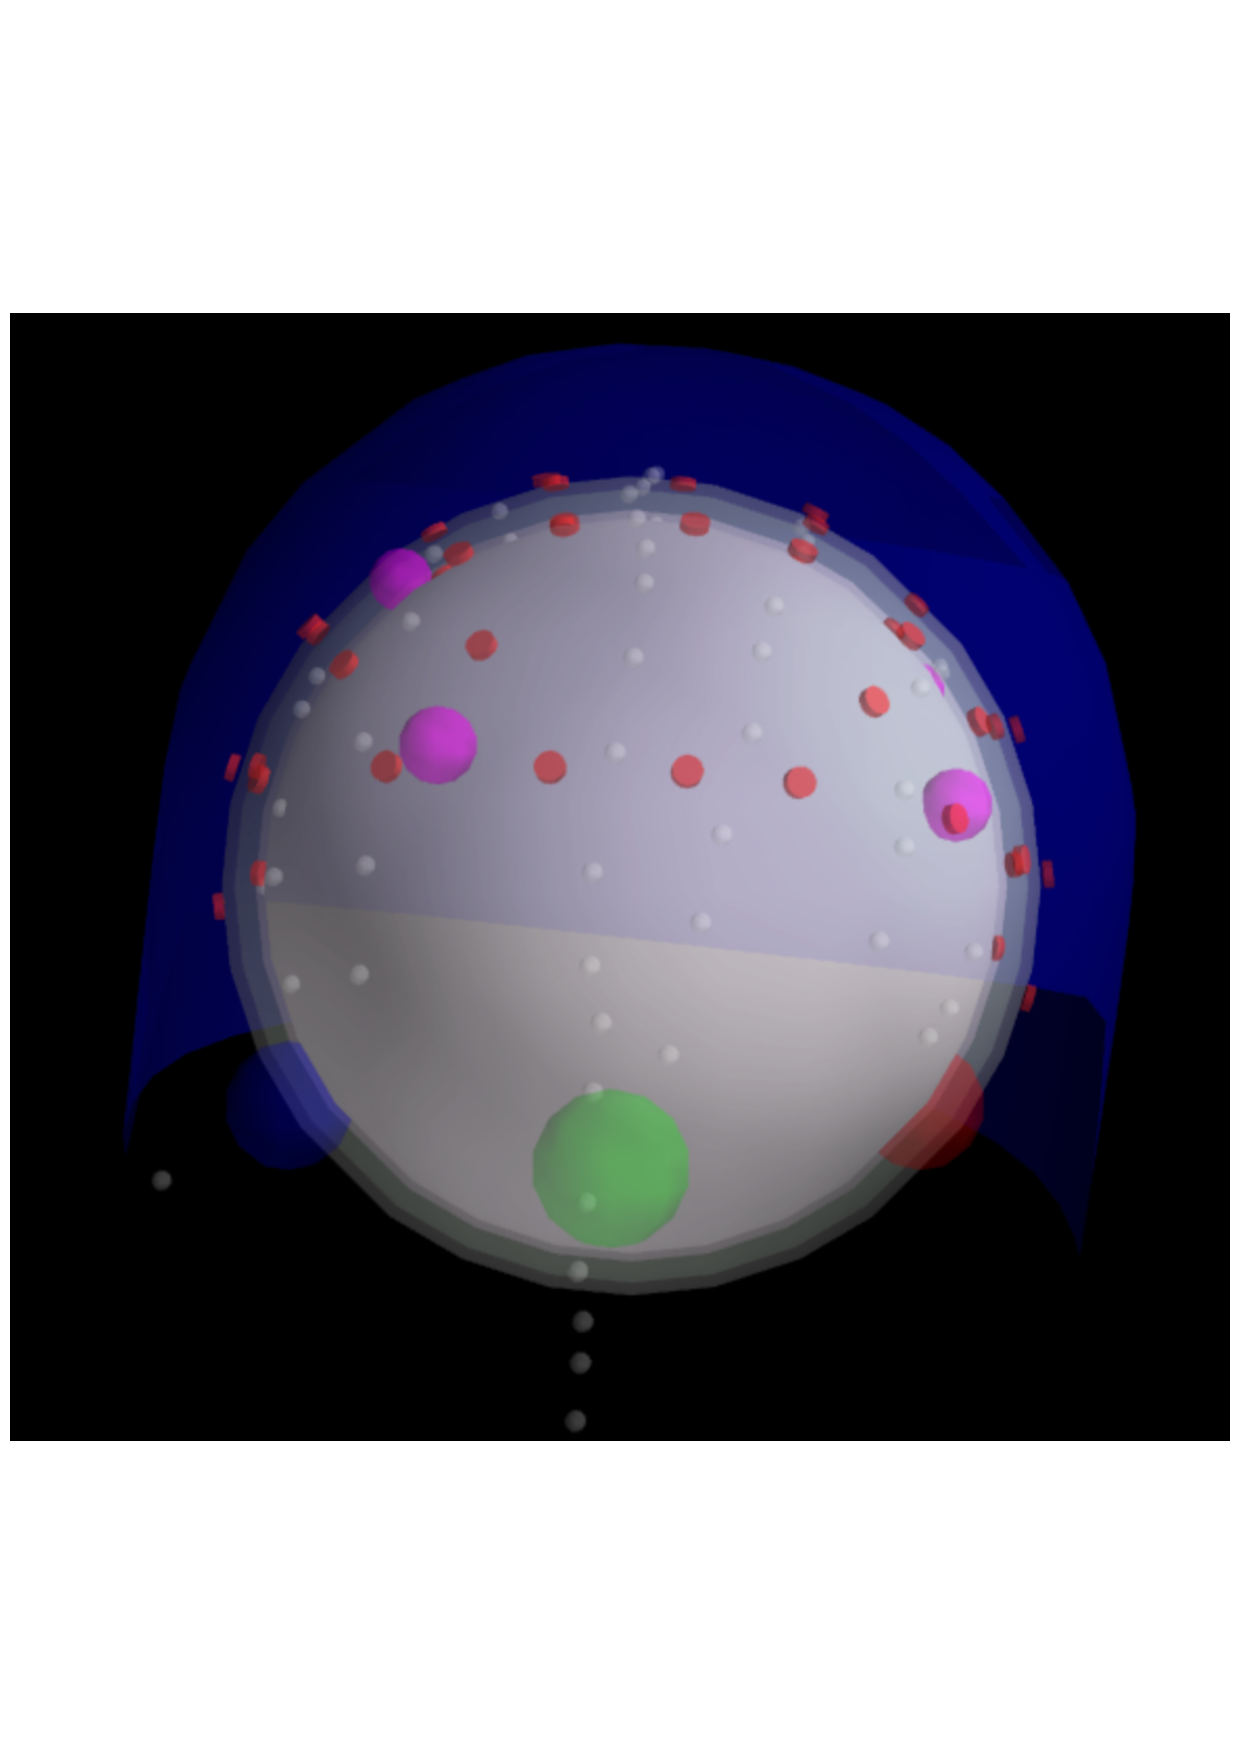
\includegraphics[trim={0cm 5cm 0cm 5cm},width=0.6\textwidth]{background/sphere_align}
    \caption{The alignment of a spherical model with three layers and the sensors. The spheres are shown in grey, the sensors space in blue, and the dots to align in order to put the spheres modeling the head and the sensors in a common coordinate system.}
	\label{fig:sphere_align}
\end{figure}

For EEG, the number and radii of the spherical layers are to be specified. Nonetheless, previous empirical work on closed-form approximations by Berg and Scherg~\cite{berg1994fast} and related theoretical studies by Zhang~\cite{zhang1995fast} have gathered a valid and convenient method for approximating an EEG field kernel from a multi-layer spherical model as the weighted sum of three kernels from a single-layer spherical model applied to a modified source configuration. The optimal values of the "Berg parameters" (Eccentricity and Magnitude) in this approximation depend on the layer radii and conductivities.

\subsection*{Realistic head models}
A more realistic head model requires that the real geometry and conductivity of the head layers be taken into account as much as possible (Figure~\ref{fig:head_model}). For real (non-spherical) geometry and conductivity fields, numerical solutions for Maxwell's equations are to be computed.\\
\begin{figure}
\centering
	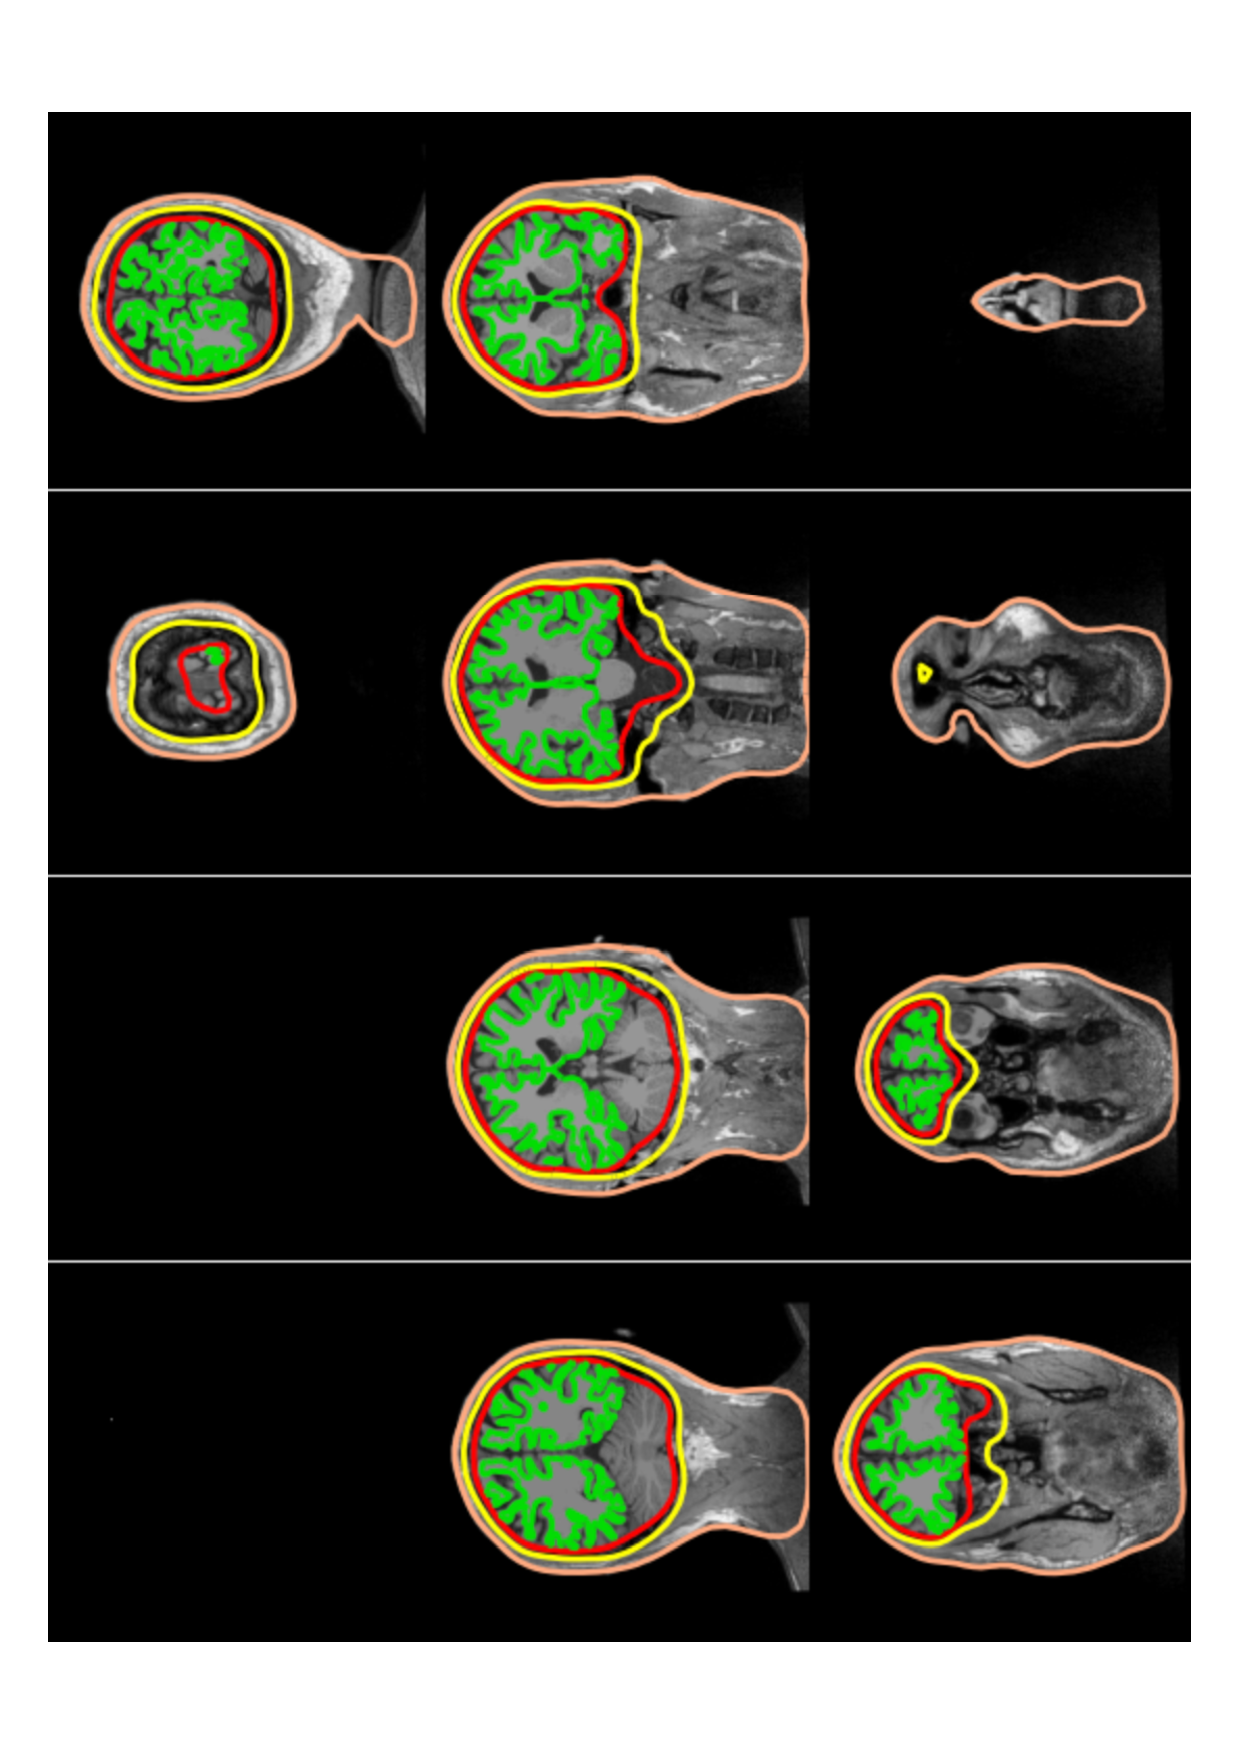
\includegraphics[angle=270,width=0.95\textwidth]{background/head_model}
    \caption{The head model: the BEM surfaces containing the three layers (inner skull, outer skull, and skin).}
	\label{fig:head_model}
\end{figure}
Assuming a piecewise constant distribution of the conductivity field, approximate, yet efficient and accurate, numeric solutions can be obtained for a realistically shaped head model using the so-called \ac{bem}. For BEM solutions, an MRI-based simplified description of the geometry is needed for computing the lead fields, and this can be provided in terms of (strictly) nested and closed surfaces corresponding to the boundaries separating the main tissue compartments (also called layers).
In practice, BEM solutions will only require to set a few conductivity parameters (one per tissue), and to specify a few triangular meshes, as can be obtained, \textit{e.g.}, with 3D volume segmentation tools from anatomical MRI data, each representing a separate interface between layers. \\

% http://leonidzhukov.net/content/eeg_meg_physics/node1.html
% http://www.brainvoyager.com/bvqx/doc/UsersGuide/EMEGSuite/EEGAndMEGForwardModels.html

%--------- MEEG inverse problem ------------------------------------------------------------
\section{The MEG/EEG Inverse problem}
An important question in the MEG/EEG community since the neuronal activity is measured at a sensor-level distributed over the head, is "how to recover the brain region(s) involved in producing the measured activity?". This is the so-called bio-electromagnetic inverse problem which is ill-posed in contrast to the forward problem. The uniqueness of the inverse problem solution is due to the fact that MEG/EEG signals can be produced by an infinite number of source configurations. Thus, to identify a stable and a unique solution among all of these infinite configurations, constraints need to be set. The constraints are chosen depending on the assumptions or a priori knowledge based on the characteristics of the source distributions, \textit{e.g.}, spatial and/or temporal characteristics of the neural activity. The source reconstruction techniques can be in general categorized as parametric (Section~\ref{section_dipfit}), scanning (Section~\ref{section_scanning}), and probabilistic methods (Section~\ref{section_distributed}).

\subsection{Parametric models: \textit{dipole fitting}} \label{section_dipfit}
Parametric methods model the problem as a small number of sources defined by their location, orientation and the strengths of the current sources that generate the MEG/EEG measurements.\\
The most common parametric method is the dipole fitting approaches \cite{scherg1985two,mosher1992multiple,scherg1990fundamentals}. It assumes that the measured data have been produced by a small number of active brain regions that can each be modeled using an equivalent current dipole (ECD). These algorithms minimize a data-fit cost function such as the Frobenius norm of the residual, and they estimate five non-linear parameters per dipole: the 3D $(x,y,z)$ position, and the two angles to define the dipole orientation. The main limitation of these methods is that they cannot be used when complex cognitive tasks are performed. This is due to the fact that the optimization problem to be solved is not linear, which implies that it gets easily trapped in local minima as soon as one tries to localize more than two dipoles. Furthermore, the number of dipoles to be estimated is not known and then needs to be set in advance. 

\subsection{Scanning methods: \textit{beamforming \& MUSIC}} \label{section_scanning}
Scanning methods, \textit{a.k.a.} beamforming, use a discrete grid to search for optimal dipole positions throughout the source space~\cite{hillebrand2005new,mosher99mulsigclassif,scherg1985two}. An estimator of the contribution of each source location to the data can be derived either via spatial filtering or signal classification settings. The simplest spatial filter is \textit{a matched filter} which uses the normalized columns of the gain matrix for spatial filtering, but the most common one is the linearly constrained minimum variance (LCMV) beamformer \cite{van1997localization}.\\
%and multiple signal classification (MUSIC) methods and their variants.\\
LCMV performs a spatial filtering on data to discriminate between signals originating from a location of interest and those coming from elsewhere, and limits the influence of the noise. In practice, it implies that the measurement matrix is multiplied by a weighting matrix. The weighting matrix should let pass signals coming from the location of interest, while attenuating signals from elsewhere. LCMV determines the weighting matrix by minimizing the output power of a filter under a constraint that its gain (forward operator) is unity at the location of interest. An attractive feature of beamforming is that it does not require any assumption on the number of the underlying sources. However it makes the strong assumption that the activations of the different sources are uncorrelated, which is not necessarily the case. An alternative to LCMV which integrates some information related to the experimental paradigms is called Synthetic Aperture Magnetometry (SAM) \cite{vrba2001signal}. Beamforming can also be applied in the frequency domain using the Dynamic Imaging of Coherent Sources (DICS) \cite{gross2001dynamic}.
%The difference between beamformers is the constraint for estimating the weighting matrix. LCMV determines the weighting matrix by minimizing the output power of a filter under a constraint that its gain is unity at the location of interest. The limitation of this approach is that signal cancellation may occur, when different sources are correlated (Baillet et al. 2001). Another beamformer often used is Synthetic Aperture Magnetometry (SAM) (Vrba and Robinson, 2001).\\

Alternatives to beamformers are methods based on signal classification using subspace decompositions. The MUltiple SIgnal Classification (MUSIC) is a widely known signal processing technique that was first applied to EEG data by \textit{Mosher} \cite{mosher1992multiple}. The primary assumptions for this method are that the dipolar time series are mutually linearly independent. 
MUSIC is based on a singular value decomposition (SVD) of the measurement data, which results in orthogonal basis vectors and singular values. Any true source localization will have a lead field (forward) vector which lies in the signal subspace computed with the SVD. MUSIC scans the brain space for source locations that satisfy this condition. The lead field vector at every candidate dipole location is systematically projected onto the signal subspace. The dipole source locations with the largest projections on the signal subspace are the active sources \cite{mosher1992multiple,mosher1999source}. However, MUSIC suffers from some problems. Firstly, when the noise present in the data is correlated across channels, MUSIC can produce larger errors in the dipole localization than would have been observed with uncorrelated noise of the same power. Another problem is the detection of multiple MUSIC peaks in a 3D space of the head, each of which may correspond to a different ECD. A related problem is to determine which peaks are truly indicative of a dipolar source rather than a local minimum in the error function \cite{mosher1999source}.

The latter problem is solved in an extended version of MUSIC, Recursively Applied and Projected (RAP)-MUSIC, by recursive estimation of multiple sources \cite{mosher1997source,mosher1999source}. In other words, it consists in applying MUSIC successively after removing the contribution of the previously identified sources. Such as matching pursuit algorithms are used for sparse signal decomposition over dictionary of atoms \cite{mallat1993matching}, the RAP-MUSIC method adopts a greedy strategy to select the relevant dipoles in a dictionary of sources. The implementation of RAP-MUSIC and its comparison with another solver was the first contribution of this thesis \cite{strohmeier-etal:16}.
%Recently, an alternative method was developed called FINES (Xu, et al., 2004). This method is able to localize closely spaced correlated sources.

\subsection{Probabilistic modeling: \textit{distributed sources \& Bayesian approaches}} \label{section_distributed}
Distributed source localization estimates the amplitudes of a dense set of dipoles distributed at fixed locations within the head surface or volume. These methods are based on the reconstruction of the brain electric activity in each point of a 3D grid of solution points, the number of points being much larger that the number of electrodes on the scalp. Each solution point is considered as a possible location of a current source, thus there is no a priori assumption on the number of dipoles in the brain.
When orientations are fixed and only the amplitudes of the sources are estimated, the forward problem results in a regression formulation.

The MEG/EEG inverse problem with distributed source models leads to a regularized regression problem. The widely known method \textit{Minimum Norm Estimate} (MNE) minimizes the $\ell_2$-norm \cite{hamalainen1994interpreting}. %The standard MNE is given in Eq.\ref{eq_thikonov}.
MNE has been very attractive due to the fact that the inverse solution is given by a simple matrix multiplication as $\ell_2$-based methods have closed-form solutions:

\begin{equation}\label{eq_MNE}
\mathbf{X}^\star = \argmin_{\mathbf{X}\in\RR^{SO\times T}} \|\mathbf{M}-\mathbf{GX}\|_{Fro}^2 + \lambda\|\mathbf{X}\|_2^2 \hspace{10pt} \mathrm{with} \hspace{10pt} \lambda > 0
\end{equation}

However, the choice of the $\lambda$ parameter as the trade-off between data fit and regularization is sometimes tricky, because it depends on the data since $\lambda$ is related to the noise level present in the measurement. $\lambda$ is most of the time chosen with a cross-validation strategy to find the optimal value in the machine learning community. While in the MEG/EEG world, it is mostly tuned by hand.

When applying a minimum-norm estimate as in Equation~\eqref{eq_MNE}, all the sources are penalized equivalently. This approach introduces bias over sources which are far from the sensors. Indeed sources which are close to the sensors have a higher forward field. Those sources are called superficial sources, and this bias is often known as the depth bias~\cite{pascual1999review}. This led to the introduction of the Weighted Minimum Norm (WMN) estimate \cite{lin2006assessing}, which downweights the dipoles in the head that are closer to the surface. 

\begin{equation}\label{eq_wMNE}
\mathbf{X}^\star = \argmin_{\mathbf{X}\in\RR^{SO\times T}} \|\mathbf{M}-\mathbf{GX}\|_{Fro}^2 + \lambda\|\mathbf{WX}\|_2^2 \hspace{10pt} \mathrm{with} \hspace{10pt} \lambda > 0
\end{equation}

$\mathbf{W}$ is a weighting matrix, which represents a priori knowledge on the source covariance. Assigning a higher variance to a deep sources is a standard approach to reduce the depth bias in MEG/EEG source imaging~\cite{lin2006assessing, TF-MxNE,haufe2008combining, haufe2011large,huang2014meg,palmero2007swloreta}. A common practice is to normalize the columns of $\mathbf{G}_s\in\RR^{S\times O}$ of the gain matrix corresponding to the $s^{th}$ source location using its Frobenius norm $\|\mathbf{G}_s\|^\delta_{Fro}$ or spectral norm $\|\mathbf{G}_s\|^\delta$~\cite{mne,TF-MxNE, kohler2006depth}. The hyperparameter $\delta$ is used to prevent a bias towards very deep sources (often fixed to $\delta=0.9$).\\

However, the current predicted inside the head with WMN as in Equation~\eqref{eq_wMNE} is very blurred. Therefore, an alternative method has been developed called FOCUSS (FOCal Underdetermined System Solution)~\cite{gorodnitsky1995neuromagnetic}. This method changes the weights at each iteration to overcome the problem. The limitation of this method is that it does not take any biophysiological information into account, and might get stuck in local minima.

Another method for the MEG/EEG inverse problem is Low Resolution brain Electromgnetic Tomography (LORETA)~\cite{pascual1994low}. This method applies $\mathbf{W}=\mathbf{L}$, where $\mathbf{L}$ is the Laplacian operator. This choice of the weighting matrix imposes neighboring sources to be correlated and thus tries to find the smoothest possible solution, however it generally provides very blurred (over-smoothed) solutions.

The dSPM~\cite{dale2000dynamic} and sLORETA~\cite{pascual2002standardized} are variants of weighted MNE which apply noise-normalized methods based on an estimate of the variance of the estimated current density. Those methods aim to represent on the cortex not the activity itself, but a \textit{dimensionless} statistical quantity depicting the significance of each source activity. The reason why dSPM has been widely used in the MEG community is the fact that using this statistical quantity reduces the bias towards the superficial sources and makes all kind of thresholding easy on the source estimate.

MNE and its variants solve the MEG/EEG inverse problem for each time point separately. They consider a spatial smoothness prior on the inverse problem, but they do not take the time dimension of the MEG/EEG data into account. Moreover they are dense models, which do not fit the assumption that only a few focal brain regions are involved in a specific cognitive task. MNE or dSPM for example will both have nonzero sources for every time instant.
For this aim, several methods favoring sparse focal source configurations have been proposed based on a relaxation of the $\ell_0$-norm. A popular approximation is $\ell_p$-norms with $0<p\leq 1$:

\begin{equation} 
\|\mathbf{X}\|_p = \Big(\sum_{s=1}^S\sum_{t=1}^T|\mathbf{X}[s,t]|^p\Big)^{\frac{1}{p}}
\end{equation} \label{eq:lp_norms}

Assuming spatially whitened MEG/EEG data, a sparse source estimate can be obtained by solving the regularized problem:

\begin{equation}
\mathbf{X}^\star = \argmin_{\mathbf{X}\in\RR^{SO\times T}} \frac{1}{2}\|\mathbf{M}-\mathbf{GX}\|_2^2 + \lambda\|\mathbf{X}\|p \hspace{10pt} \mathrm{with} \hspace{10pt} \lambda > 0.
\end{equation} \label{eq:regularized_problem}

The optimization problem is non-differentiable, and has no a closed-form solution. Hence iterative approaches need to be applied to solve the problem in Equation~\eqref{eq:regularized_problem}. Fixing $p=1$ in Equation~\eqref{eq:regularized_problem}, the problem is known as \ac{lasso}~\cite{Tibshirani96} in statistics, Basis Pursuit Denoising (BPDN)~\cite{Chen_Donoho_Saunders98} in signal processing, and Selective Minimum Norm (SMN)~\cite{matsuura1995selective} in MEG/EEG. However applying the $\ell_1$-norm for the free or the loose orientation ($O=3$) promotes sparsity even within the orientation at each source location. To overcome this issue, Minimum Current Estimate (MCE) has been proposed by~\cite{Uutela-etal:1999} solving SMN by fixing the orientation priori by computing first a MNE solution. \\

Several other approaches can be cited that investigate the same idea of having focal source estimates. Sparse Bayesian Learning (SBL)~\cite{wipf2006bayesian}, Spatio-Temporal TOmographic NonNegative Independent Component Analysis (STTONNICA)\cite{valdes2009eeg}, mixed-norms~\cite{ou2009distributed}, Champagne~\cite{owen2012performance}, hierarchical Bayesian inference\cite{lucka2012hierarchical}, or the Mixed-Norm estimates (MxNE)~\cite{gramfort2012mixed}. Those methods are called spatio-temporal because they work in a predefined time window, however they completely ignore the temporal correlation. This can be verified by shifting the columns of the source estimate: it will have no effect on the source estimate itself. \\

To introduce a "true" spatio-temporal constraint in the model, \cite{zhang2011sparse,zhang2011iterative} incorporated the temporal correlation to improve the source estimates, the vector-based spatio-temporal minimum $\ell_1$-norm solver (VESTAL)~\cite{huang2006vector} applies a temporal projection to reduce the sensitivity to noise after using the $\ell_1$-norm. The fast-VESTAL~\cite{huang2014meg} is a sort of postprocessing to the VESTAL method. The Fast-VESTAL technique consists of two steps. First, $\ell_1$-minimum-norm MEG source images were obtained for the dominant spatial modes of sensor-waveform covariance matrix. Next, accurate source time-courses with millisecond temporal resolution were obtained using an inverse operator constructed from the spatial source images of the first step. However this postprocessing step implicitly assumes that the source estimates are stationary. To overcome these issues, Ou et al.~\cite{Ou-etal:2009} proposed an approach to reconstruct multiple time instants simultaneously by applying the $\ell_{2,1}$-mixed-norm to impose group sparsity as a spatio-temporal regularization~\cite{gramfort2012mixed,Ou-etal:2009}.

The Time-Frequency Mixed-Norm Estimate (TF-MxNE) solver~\cite{TF-MxNE} reused the $\ell_{2,1}$-mixed-norm (MxNE) in the time-frequency domain by adding a second regularization over time ($\ell_{2,1} + \ell_1$). It multiplies the gain matrix by a dictionary of spatial basis functions. They obtain a modified gain matrix, which can be used to estimate spatially extented sources with temporally smooth waveforms. This approach was also investigated by~\cite{castano2015solving}, calling the method Spatio-Temporal Unifying Tomography (STOUT).

Although these spatio-temporal methods improve the MEG/EEG source reconstruction, they are based on convex penalties. This allows fast algorithms with guaranteed global convergence. However, the resulting source estimates are biased in amplitude and often suboptimal in terms of support recovery, \textit{i.e.}, active sources \cite{candes2008enhancing}. As shown \textit{e.g.} in the field of compressed sensing, promoting sparsity by applying non-convex penalties, such as logarithmic or  $\ell_p$-quasinorm penalties with $0<p<1$, improves support reconstruction in terms of feature selection, amplitude bias, and stability~\cite{candes2008enhancing,chartrand2007exact,saab2008stable}. Several approaches for solving the resulting non-convex optimization problem have been proposed, including iterative reweighting $\ell_1$ optimization \cite{candes2008enhancing}. \cite{strohmeier2014iterative} used an iterative reweighted approach to solve the composite non-convex penalty in the time-frequency domain.

%\textbf{Local autoregressive average (LAURA)}\\
%\textbf{EPIFOCUS}\\

%\subsection{Minimum norm solutions and its \textit{sparse} variants}
%\subsection{Other methods}
%\textbf{Bayesian method}\\
%\textbf{ELECTRA}\\

%https://books.google.fr/books?id=s1VfR1T3P08C&pg=PA85&lpg=PA85&dq=inverse+problem+meg+book+bird+image&source=bl&ots=dZ-XzI5x7M&sig=1TVAsYPk1t4AD_XzyeGqduIp97s&hl=en&sa=X&ved=0ahUKEwikzKrVi6_MAhWCUBQKHRqQAwwQ6AEIIzAB#v=onepage&q&f=false

%http://www.fil.ion.ucl.ac.uk/~wpenny/publications/spm-book/steeg.pdf

%https://books.google.fr/books?id=YLyGmfVuBsIC&pg=PA192&lpg=PA192&dq=inverse+problem+meg+book&source=bl&ots=q2QE3dxz__&sig=OElFKShtnznrpaCeLHZMbTAOBmw&hl=en&sa=X&ved=0ahUKEwj95bm9iq_MAhWCvxQKHWCeA3MQ6AEIWjAI#v=onepage&q=inverse%20problem%20meg%20book&f=false

\subsection{Conclusion}
This part has presented an overview on the state of the art of the MEG and EEG inverse solvers. Although multiple solvers have been provided, this list is definitely not exhaustive.
We have kept at the end the distributed solvers which are the main interest of this thesis. Here, we will model the problem as a regularized regression with sparse priors. In the next part of the chapter, we discuss all aspects of linear regression, different penalization terms, especially the ones promoting sparsity, and the algorithms for solving those optimization problems.

%-----------------Time-Frequency------------------------------------------------------------
\section{Time-Frequency representation}
\label{section:TF}
% http://www.dafx.ca/slides/keynote1.pdf
In signal processing, time-frequency analysis encompasses those techniques that study a signal in both time and frequency domains simultaneously, using various \ac{TFR}. During the last decades, the signal processing community has provided many new techniques for expanding signals into "elementary" waveforms, such as wavelet bases, \ac{MDCT}, short time Fourier transform (STFT), Gabor wavelets (frames), etc. More often, the key issue is to obtain a sparse representation of the signal, when it is better defined in the frequency domain than the time domain. For example, a sine wave is sparsely represented in the Fourier domain, not in the time domain.\\

A signal representation is sparse when most information is concentrated in a small amount of data or coefficients. Several applications such as denoising make use of the sparse TFR because the noise is not sparse: source separation, signal modeling, etc. A key ingredient is to decompose a signal into a linear combination of "elementary" waveforms $\psi_{i}$:
\begin{equation}\label{eq_signal_decomp}
x(t) = \sum_i\alpha_i\psi_i(t)
\end{equation}
with $\alpha_i$ the coefficients, and $\psi_i$ the waveforms. See \cite{mallat2008wavelet,hlawatsch1992linear,wickerhauser1994adapted} for detailed examples of signal representations.\\

\subsection{Modified Discrete Cosine Transform: MDCT} \label{section:mdct}
The mathematically simplest tool for signal decomposition is based on orthonormal bases. The waveform system $\mathcal{W}=\{\psi_i, i \in\Lambda\}$ is an orthonormal basis of the signal space (assumed to be a Hilbert space with an inner-product) $\mathcal{H}$ is:
\begin{itemize}
\item The atoms are mutually orthogonal and normalized: $\langle\psi_i,\psi_j\rangle = 0$ and $\|\psi_i\|=1$
\item They form a complete set of $\mathcal{H}$: if the signal $x\in\mathcal{H}$ is such that $\langle x,\psi_i\rangle=0$ for all $i\in\Lambda$, then $x=0$.
\end{itemize}
Then, any signal can be written in a unique way as in Equation~\eqref{eq_signal_decomp} with $\alpha_i=\langle x,\psi_i\rangle$.\\

MDCT basis vectors are shift variant and its coefficients are real valued. They cannot be easily interpreted in terms of magnitude and phase.

\subsection{Gabor dictionaries} \label{section:gabor}
Given a signal observed over a time interval, its conventional Fourier transform computes the frequency content but loses the time information. To analyze the evolution of the spectrum over time and hence the non-stationarity of the signal, Gabor introduced windowed Fourier atoms which correspond to a \ac{STFT} with a Gaussian window. In practice, for numerical computation, a challenge is to properly discretize the continuous STFT. The discrete STFT with a Gaussian window is also known as the discrete Gabor Transform \cite{gabor1946theory}.

The setting we consider is the finite-dimensional one. Let $\mathbf{g}\in \RR^{T}$ be a "mother" analysis window. Let $f_0\in \mathbb{N}$ and $k_0\in \mathbb{N}$ be the frequency and time sampling rates in the time-frequency plane generated by the STFT, respectively. The family of the translations and modulations of the mother window generates a family of Gabor atoms $(\mathbf{\phi}_{mf})_{mf}$ forming the dictionary $\mathbf{\Phi}\in \mathbb{C}^{T\times C}$, where $C$ denotes the number of atoms. The atoms can be written as:
\begin{equation} \label{eq_gabor_atoms}
	\mathbf{\phi}_{mf}[n] = \mathbf{g}[n-mk_0]e^{\frac{i2\pi f_0 fn}{T}}, m\in \{0,\dots ,\frac{T}{k_0}-1\}, f\in \{0,\dots ,\frac{T}{f_0}-1\}.
\end{equation}
If the product $f_0k_0$ is small enough, \textit{i.e.}, the time-frequency plane is sufficiently sampled, the family $(\mathbf{\phi}_{mf})_{mf}$ is a frame of $\RR^T$, \textit{i.e.}, one can recover any signal $\mathbf{x}\in \RR^T$ from its Gabor coefficients $(\langle \mathbf{x}, \mathbf{\phi}_{mf}\rangle)=\mathbf{\Phi}^{\mathcal{H}}\mathbf{x}$. More precisely, there exists two constants $A, B > 0$ such that:
\begin{equation} \label{eq_frame}
	A\|x\|_2^2 \leq \sum_{m,f}|\langle \mathbf{x}, \mathbf{\phi}_{mf}\rangle|^2\leq B\|x\|_2^2 \enspace .
\end{equation}
When $A=B$, the frame is \textit{tight}. When the vectors $\mathbf{\phi}_{mf}$ are normalized, the frame is an orthogonal basis if and only if $A=B=1$. The Balian-Low theorem says that it is impossible to construct a Gabor frame which is a basis. Consequently, a Gabor transform is redundant or overcomplete and there exists an infinite number of ways to reconstruct $\mathbf{x}$ from a given family of Gabor atoms. In the following, the considered $\mathbf{\Phi}$ dictionaries are tight frames.

The canonical reconstruction of $\mathbf{x}$ from its Gabor coefficients requires a canonical dual window, denoted by $\mathbf{\tilde{g}}$. Following Equation \eqref{eq_gabor_atoms} to define $(\tilde{\mathbf{\phi}}_{mf})_{mf}$ we have:
\begin{equation} \label{eq_TF_recons}
	\mathbf{x}=\sum_{m,f}\langle\mathbf{x}, \mathbf{\phi}_{mf}\rangle\tilde{\mathbf{\phi}}_{mf}=\mathbf{\Phi}^{\mathcal{H}}\mathbf{x\tilde{\Phi}}=\tilde{\mathbf{\Phi}}^{\mathcal{H}}\mathbf{x\Phi},
\end{equation}
where $\tilde{\mathbf{\Phi}}$ is the Gabor dictionary formed with the dual windows. If the frame is tight, then we have $\tilde{\mathbf{g}}=\mathbf{g}$, and more particularly we have $\mathbf{\Phi\Phi}^{\mathcal{H}}=\|\mathbf{\Phi\Phi}^{\mathcal{H}}\|\mathbf{I}$. The representation being redundant, for any $\mathbf{x}\in\RR^T$ one can find a set of coefficients $z_{mf}$ such that $\mathbf{x}=\sum_{m,f}z_{mf}\mathbf{\phi}_{mf}$, while the $z_{mf}$ verify some suitable properties dictated by the application. For example, it is particularly interesting for MEG/EEG to find a sparse representation of the signal. Indeed, a spectrogram, sometimes simply called TF transform of the data in the MEG literature, generally exhibits a few peaks localized in the time-frequency domain. In other words, MEG/EEG signals can be expressed as linear combinations of a few oscillatory atoms. In order to demonstrate this, Fig. \ref{fig:stft} shows the STFT of a single signal from a MEG channel from a somatosensory experiment, the same STFT restricted to the 50 largest coefficients (approximately only 10\% of the coefficients), and the signal reconstructed with only these coefficients compared to the original signal. We observe that the original signal can be very well approximated by only a few coefficients, \textit{i.e.}, a few Gabor atoms.

\begin{figure}
\centering
	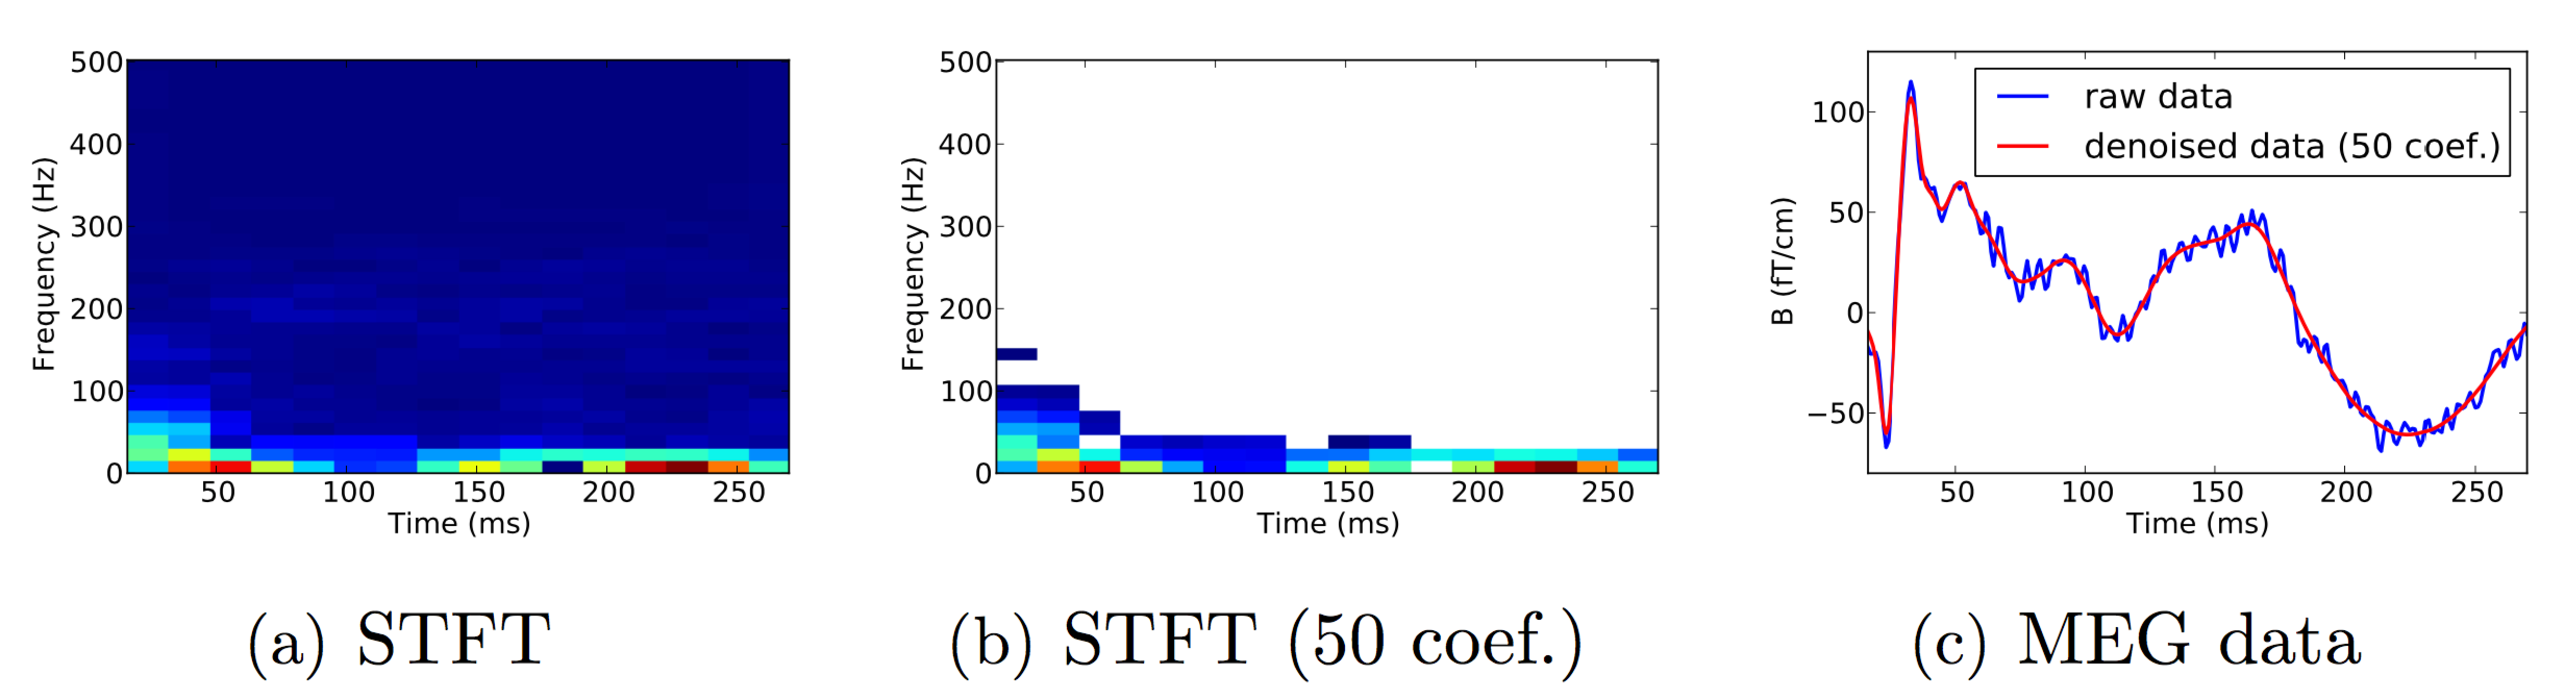
\includegraphics[width=\textwidth]{background/stft}
    \caption{a) STFT of a single channel MEG signal sampled at 1000Hz showing the sparse nature of the transformation (window size 64 time points and time shift $k_0=16$ samples). b) STFT restricted to the 50 largest coefficients. c) Original data and reconstructed data using only the 50 largest coefficients.}
	\label{fig:stft}
\end{figure}

In practice, the Gabor coefficients are computed using the Fast Fourier Transform (FFT) and not by a multiplication by a $\mathbf{\Phi}$ matrix as suggested above. Such operations can be efficiently implemented as in the LTFAT toolbox\footnote{http://ltfat.sourceforge.net} \cite{sondergaard2012linear}. Another practical concern to keep in mind is the trade-off between the size of the window $\mathbf{g}$ and the time shift $k_0$. A long window will have a good frequency resolution and a limited time resolution. The time precision can be improved with a small time shift, leading however to a larger computational cost, both in time and memory. Finally as any computation done with an FFT, the STFT implementations assume circular boundary conditions for the signal. To take this into account and avoid edge artifacts, the signal has to be windowed.\\

For more details about Gabor dictionaries, please refer to \cite{daubechies1992ten}.

\subsection{Conclusion}

This last part briefly introduced some important properties of time-frequency representations. It presented MDCT and Gabor dictionaries. It mainly explained the advantage of using the tight Gabor frames concept. The STFT or Gabor frames are time invariant, contrary to MDCT. Chapter~\ref{chapter:multiscale} will model the inverse problem in the \ac{TF} domain, which is based on the construction of Gabor frames. 

%-----------------Optimization--------------------------------------------------------------
\section{Optimization}
Due to the fact that the MEG/EEG sensors are linear combinations of the electromagnetic fields produced by all current sources, the linear forward operator, called \textit{gain matrix}, or the \textit{mixing matrix}, predicts the MEG/EEG measurements. Here we introduce the linear regression on which the formulation of the MEG/EEG inverse problem is based in this thesis.

\subsection{Linear model and regression}
%\textbf{XXX: intro to convexity...}
In statistics, linear regression consists of modeling the linear relationship between an observation $\textbf{y}$ and some explanatory variables $\mathbf{A}=[A_1,\dots ,A_n]^\top$. This relationship involves the vector of coefficients $\mathbf{x}\in\RR^m$ such that:
\begin{equation} \label{eq_linreg}
	y = Ax	
\end{equation}
% \langle\mathbf{s}, \mathbf{x}\rangle = y \enspace .
This linear model is verified for a set of observations coming from the same event, \textit{i.e.} the linear combination defined by $\mathbf{x}$ is the same for all (variable, observation) couples originating from the same event: $(\mathbf{A}_i, y_i)\in\RR^m\times\RR$ with $i\in [1,\dots ,n]$. We can note $[y_1, \dots ,y_n]^\top=\mathbf{y}\in\RR^n$ and $[\mathbf{A}_1,\dots ,\mathbf{A}_n]\in\RR^{m\times n}$. If all couples $\{(\mathbf{A}_i,y_i)\}_{i\in [1,\dots ,n]}$ verify exactly a linear model, then there exists a vector $\mathbf{x}\in\RR^m$ such that $\mathbf{Ax}=\textbf{y}$.

In a MEG/EEG application, the equivalent of $\mathbf{A}$ is the forward operator $\mathbf{G}$ which describes the linear relationship between the MEG/EEG measurements $\mathbf{M}\in\RR^{N\times T}$ ($N$ number of sensors, $T$ number of time instants) and the source activation $\mathbf{X}\in\RR^{S\times T}$ ($S$ is the number of source locations). The linear model then reads: $\mathbf{M} = \mathbf{GX}$ where $\mathbf{G}\in\RR^{N\times S}$ is the gain or the lead-field matrix (forward operator), a known instantaneous mixing matrix, which links source and sensor signals. 

In practice, the linear model is never exactly verified due to external noise. The aim of linear regression is to additionally assume that an unobserved random variable, \textit{i.e.} error term, is added to the linear relationship between the M/EEG measurements $\mathbf{M}$ and the source activation $\mathbf{X}$. The regression model can then be written similarly to Equation~\eqref{eq:meeg_ip}:
\begin{equation} \label{eq_linmeeg}
	\mathbf{M} = \mathbf{GX} + \mathbf{E}
\end{equation}
with $\mathbf{E}$ is the measurement noise, which is assumed to be additive, white, and Gaussian, \mbox{$\mathbf{E}_{.,j}\sim\mathcal{N}(0,\mathbf{I})$} for all $j$. This assumption is acceptable on the basis of a proper spatial whitening of the data using an estimate of the noise covariance \cite{engemann2015automated}.

Several methods exist to approximate the solution of the regression model. The most widely used is the \ac{OLS} approach \cite{legendre1805nouvelles}, which minimizes the sum of the squares of the errors or residuals as follows:
\begin{equation} \label{eq_ls}
	\mathbf{X^\star} \in \argmin_{\mathbf{X}\in \RR^{S\times T}}\frac{1}{2} \|\mathbf{M}-\mathbf{GX}\|_{Fro}^2
\end{equation}
There exist other types of approaches like the \ac{LAD}, also known as least absolute errors. Instead of minimizing the squares of the errors, \ac{LAD} tries to minimize the sum of the absolute values of the errors/residuals. Its advantage over \ac{OLS} is that it is more robust to outliers in the data. However the LAD is not stable, \textit{i.e.}, a small modification of the observation $\mathbf{M}$ may result in a huge variation of the estimation of $\mathbf{X}$. Moreover it can have multiple solutions, because unlike \ac{OLS}, it does not have an analytical expression but needs to be computed iteratively. This explains why the OLS approach has been the standard one, along with the fact that it has a closed-form solution.

\subsection{Regularization}

Regularization in general can be applied for different reasons. We have seen why the least squares is the standard approach in linear regression. However this approach has some drawbacks: \textit{overfitting} \footnote{Overfitting: when the model fits the training data too well and has bad generalization} and the fact that the closed-form solution is computed using $\mathbf{G}^\top\mathbf{G}$, which might not be invertible, giving rise to infinitely many solutions. This requires to set regularization.\\

In general, the penalization term will be marked $\mathcal{P}(\mathbf{X})$ as in Equation~\eqref{eq_reg} and it can take any dense or sparse form:
\begin{equation} \label{eq_reg}
	\mathbf{X}^\star = \argmin_{X\in\RR^{S\times T}}\frac{1}{2}\|\mathbf{M}-\mathbf{GX}\|_{Fro}^2 + \lambda\mathcal{P}(\mathbf{X})
\end{equation}
In the rest of this section, we list the different regularization terms $\mathcal{P}(\mathbf{X})$ as those using: dense norms, convex sparse norms, non-convex sparse norms, and structured norms.

\subsubsection*{Non-sparsity promoting norms}
Thikonov regularization \cite{tikhonov1977solutions} is the most commonly used penalty, also known as rigde regression \cite{hoerl1970ridge}. It is part of dense norms as the estimated $\mathbf{X}^\star$ is dense, even if most of its values are almost zero. It reads:
\begin{equation} \label{eq_thikonov}
	\mathbf{X}^\star = \argmin_{X\in\RR^{S\times T}}\frac{1}{2}\|\mathbf{M}-\mathbf{GX}\|_{Fro}^2 + \lambda\|\mathbf{X}\|_2^2
\end{equation}

The first term of the minimization is called the data fit, and the second term penalizes the solution by keeping the values of $\mathbf{X}$ small. We always keep the same data fit term $\frac{1}{2}\|\mathbf{M}-\mathbf{GX}\|_{Fro}^2$ and change the second penalization term depending on our priori knowledge. The penalization is controlled by the $\lambda$ parameter. The higher it is, the more penalized the regression is. An explicit solution of Equation~\eqref{eq_thikonov} is given by $\mathbf{X}^\star = (\mathbf{G}^\top\mathbf{G}+\lambda\mathbf{I})^{-1}\mathbf{G}^\top\mathbf{M}$. 

In this thesis, we are interested in sparsity promoting regularizations, which are natural for the MEG/EEG inverse problem. Indeed, it is reasonable to assume that only a few focal regions in the brain are active during a certain cognitive task.

\subsubsection*{Sparse norms: \textit{Convex norms}}
Let $\mathbf{y}\in\RR^n$ a vector. The support of $y$ is defined by the set $\mathcal{S}(y) = \{i=[1,\dots ,n] \mathrm{\ s.t.\ } \\ y[i]\neq 0\}$.
A vector is sparse if its support is small, \textit{i.e.} the cardinal $\# \mathcal{S}(y)$ is small compared to $n$.
The cardinal of $\mathcal{S}(y)$ corresponds to the $\ell_0$ pseudo-norm. The optimization problem implies then to identify $\mathcal{S}(y)$.\\

Coming back to our application, we assume that the signals $\mathbf{M}$ obtained with MEG/EEG are linear combinations of a small number of sources in the brain. This implies that only few sources in $\mathbf{X}$ are active, \textit{i.e.}, $\mathbf{X}$ is sparse. However the minimization of Equation~\eqref{eq_reg} with the $\ell_0$-norm ($\mathcal{P}(\mathbf{X})=\|\mathbf{X}\|_0$) is unfortunately an NP-hard combinatorial problem.
% This problem is difficult as we need to select the the number of sources. Furthermore, the $\ell_0$-norm is not convex \cite{natarajan1995sparse}.

Due to the above undesired properties, we need to consider a convex relaxation of the $\ell_0$-norm. The use of the least squares with the $\ell_1$-norm (i.e. $\mathcal{P}(\mathbf{X})=\|\mathbf{X}\|_1$ in Equation~\eqref{eq_reg}) is the natural approximation, since it is the closest convex norm to the $\ell_0$-norm. The $\ell_1$-norm is known as \textit{\ac{lasso}} in statistics \cite{tibshirani1996regression}, and as Basis Pursuit Denoising~\cite{chen2001atomic} in signal processing literature.

\adjustwidth{1em}{0pt}
\subsubsection*{\ac{lasso}}
\begin{equation} \label{eq_lasso}
	\mathbf{X}^\star = \argmin_{\mathbf{X}\in\RR^{S\times T}}\frac{1}{2}\|\mathbf{M}-\mathbf{GX}\|_{Fro}^2 + \lambda\|\mathbf{X}\|_1
\end{equation}
\endadjustwidth
The use of a convex approximation of the $\ell_0$-norm is convenient, as the method always converges to a globally optimal solution. There exist also very efficient algorithms.

\subsubsection*{Sparser norms: \textit{Non-Convex norms}}
These convex approaches allow for fast algorithms with guaranteed global convergence. However, the resulting source estimates are biased in amplitude and often suboptimal in terms of support recovery~\cite{candes2008enhancing}. This is particularly due to the high spatial correlation of the MEG/EEG forward model. As shown, \textbf{e.g.} in the compressed sensing literature, promoting sparsity by applying non-convex penalties, such as logarithmic or $\ell_p$-quasinorm penalties with $0 < p < 1$, can improve support identification, as well as reduce amplitude bias~\cite{candes2008enhancing,chartrand2007exact,saab2008stable}. Figure~\ref{fig:norms} shows the geometric interpretation of different norms in the 1-dimensional space. The smaller $p$, the closer is this approximation to the exact definition of sparsity. 

\begin{figure}
\centering
	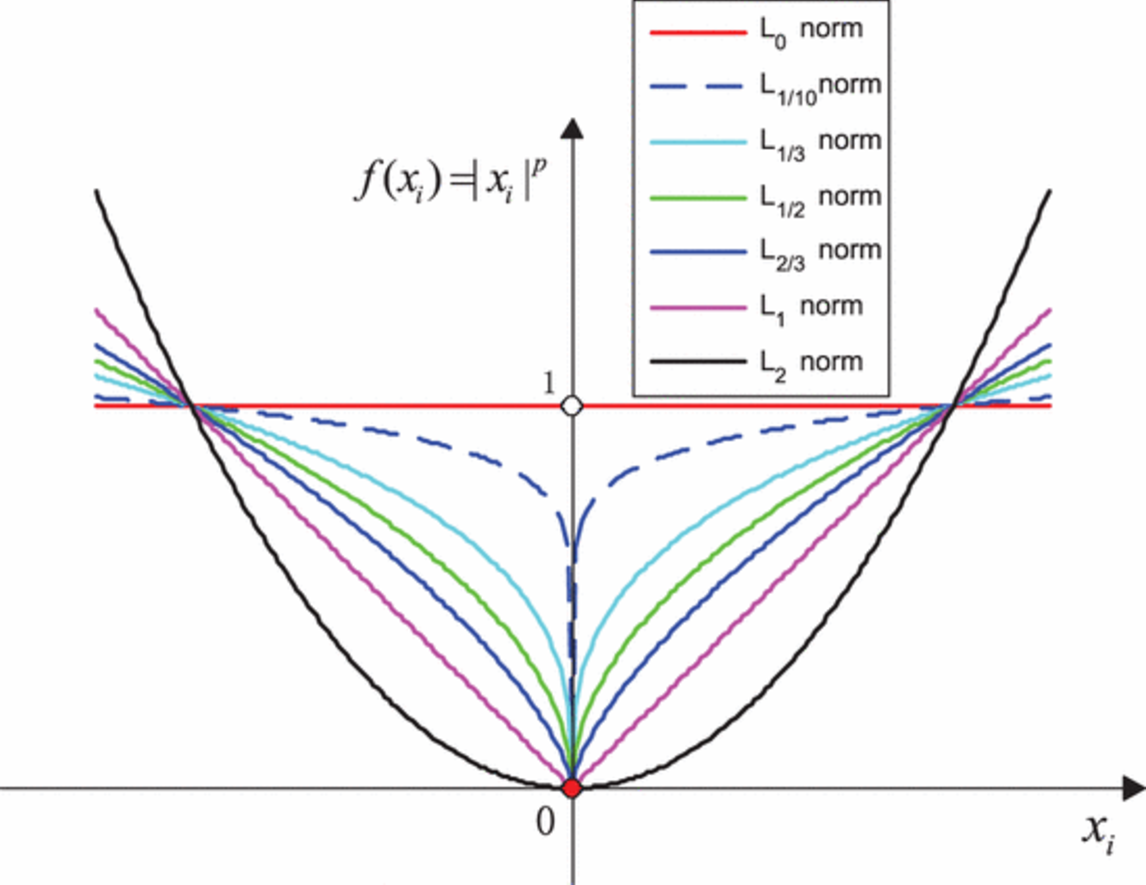
\includegraphics[width=0.7\textwidth]{background/norms}
	%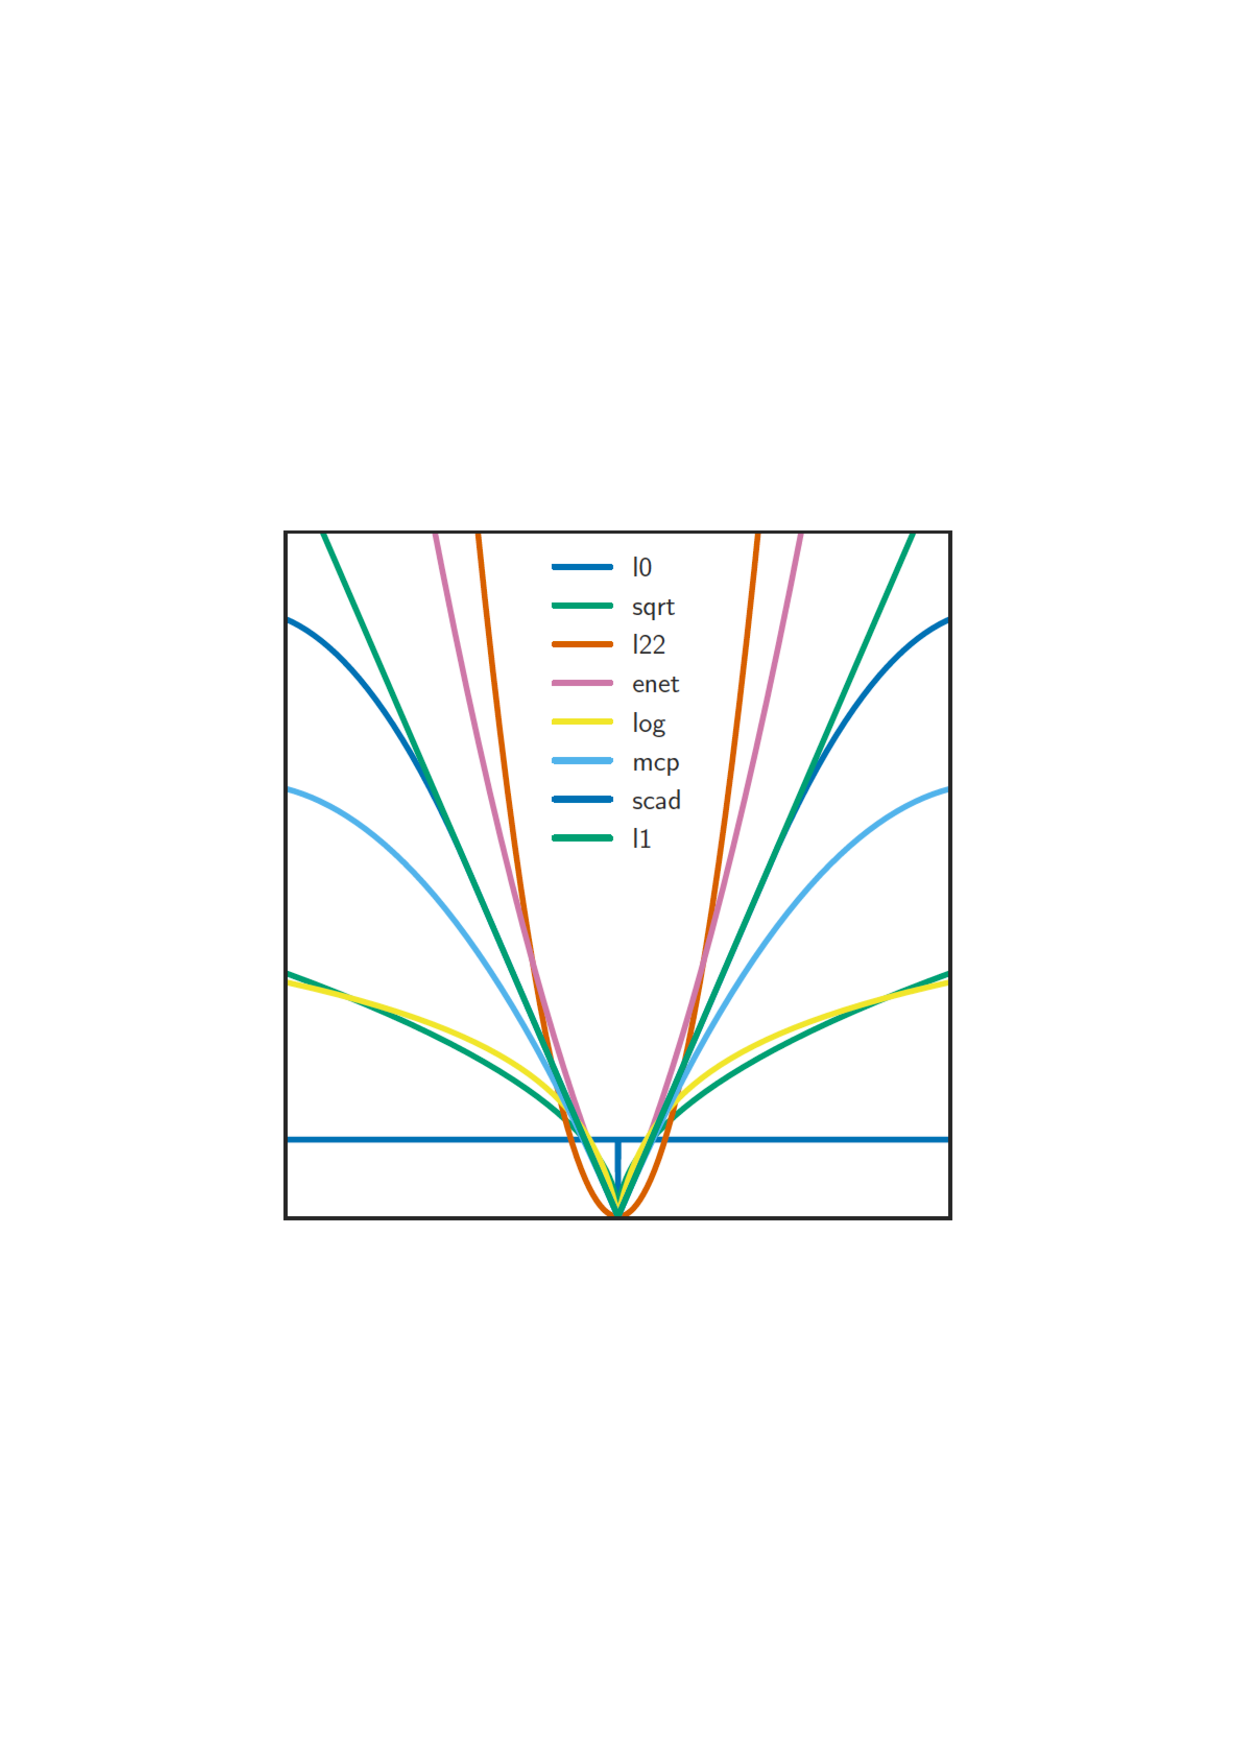
\includegraphics[trim={1cm 8cm 2cm 8cm},width=0.6\textwidth]{background/norms_methods}
    \caption{Geometric interpretation of the different norms in 1D space.}
	\label{fig:norms}
\end{figure}

We investigated the $\ell_{0.5}$-quasinorm as part of the regularization, written as:
\adjustwidth{1em}{0pt}
\subsubsection*{$\ell_{0.5}-quasinorm$}
\begin{equation} \label{eq_quasinorm}
	\mathbf{X}^\star = \argmin_{\mathbf{X}\in\RR^{S\times T}}\frac{1}{2}\|\mathbf{M}-\mathbf{GX}\|_{Fro}^2 + \lambda\|\mathbf{X}\|_{0.5}
\end{equation}
\endadjustwidth

As the $\ell_{0.5}$-quasinorm is non-convex, it cannot be solved in the same way and with the same guarantees as the $\ell_1$-norm. One algorithm for solving Equation~\eqref{eq_reg} using the $\ell_{0.5}$ quasi-norm consists in applying an iterative reweighted approach, where each iteration boils down to a convex problem with a weighted $\ell_1$ regularization.
\adjustwidth{1em}{0pt}

\subsubsection*{Weighted \ac{lasso}}
\begin{equation} \label{eq_wlasso}
	\mathbf{X}^\star = \argmin_{\mathbf{X}\in\RR^{S\times T}}\frac{1}{2}\|\mathbf{M}-\mathbf{GX}\|_{Fro}^2 + \lambda\|\mathbf{X}\|_{\mathbf{W};1}
\end{equation}
with
\begin{equation*}
	\|\mathbf{X}\|_{\mathbf{W};1}=\sum_i\sum_j W[i,j]|X[i,j]|
\end{equation*}
where $\mathbf{W}$ is the weight applied to matrix $\mathbf{X}$ aiming to regularize more the low coefficients, resulting in a higher sparsity. The update of the weight $\mathbf{W}$ will be presented in Chapter \ref{chapter:multiscale}.
\endadjustwidth

\subsubsection*{Structured Norms: \textit{non stationary sources in TF domain}}\label{sec:mixed_norms}
In some applications, like for MEG/EEG, one is not only interested in sparsity, as a-priori knowledge is available on the structure of the support of $\mathbf{X}$. To go beyond the sparsity with the $\ell_p$-norms where $0<p<1$, \cite{yuan2006model} introduced the Group \ac{lasso} in order to take grouped structures  in the data into account. It uses a mixed $\ell_2$ and $\ell_1$-norm on $\mathbf{X}$. The idea is to keep a small number of groups active ($\ell_1$) but once a group is active, then the coefficients of that group will be all nonzero ($\ell_2$).
\adjustwidth{1em}{0pt}
\vspace{-10pt}
\subsubsection*{Group \ac{lasso}}
\vspace{-10pt}
\begin{equation} \label{eq_glasso}
	\mathbf{X}^\star = \argmin_{\mathbf{X}\in\RR^{S\times T}}\frac{1}{2}\|\mathbf{M}-\mathbf{GX}\|_{Fro}^2 + \lambda\|\mathbf{X}\|_{2,1}
\end{equation}
where
\begin{equation*}	\|\mathbf{X}\|_{2,1}=\sum_i\left(\sum_j|X[i,j]|^2\right)^{1/2}
\end{equation*}
\endadjustwidth
While the Group \ac{lasso} gives only a sparse set of groups, sometimes we would like to obtain sparsity in groups and within each group. In our application, a group is basically a source, \textit{i.e.} a position in the brain. The Group \ac{lasso} is definitely convenient to obtain sparse source estimates, however it is not efficient for sources which are active only during small time windows. Toward this end, one can use Sparse Group \ac{lasso}~\cite{simon2013sparse}, which is a convex combination of the \ac{lasso} and the Group \ac{lasso} penalties.
\adjustwidth{1em}{0pt}

\subsubsection*{Sparse Group \ac{lasso}}
\begin{equation} \label{eq_sglasso}
	\mathbf{X}^\star = \argmin_{\mathbf{X}\in\RR^{S\times T}}\frac{1}{2}\|\mathbf{M}-\mathbf{GX}\|_{Fro}^2 + \lambda_1\|\mathbf{X}\|_{2,1} + \lambda_2\|\mathbf{X}\|_1
\end{equation}
If $\lambda_1=0$ then it would be equivalent to the \ac{lasso} penalty, and if $\lambda_2=0$, it results in the Group \ac{lasso} penalty.
\endadjustwidth

%----------Methods for solving sparse inverse problems-------------------------------------
\subsection{Methods for solving sparse inverse problems}
The previous section describes the MEG/EEG inverse problem as a penalized regression model. This section enumerates some methods for solving this inverse problem using sparse priors. The corresponding MEG/EEG inverse solver for the $\ell_1$-norm is the MCE solver (Minimum Current Estimate) introduced by Matsuura and Okabe \cite{matsuura1995selective}. One possible way to solve the $\ell_1$ penalty is to use the Iterative Least Squares (IRLS). IRLS consists in iteratively computing weighted LS by setting appropriate weights. This is based on the fact that a weighted $\ell_2$-norm: $\|\mathbf{x}\|_{\mathbf{w};2}=\sum_i w[i]^k |x[i]|^2$ is equal to the $\ell_1$-norm: $\|x\|_1=\sum_i|x[i]|$, when $w[i]^k=1/|x[i]|$, where $k$ denotes the iteration index. This corresponds to WMN in Section~\ref{section_distributed}. Similar iterative weighted methods are used to solve the (Sparse) Group \ac{lasso} corresponding to mixed-norms in both standard and time-frequency domains presented in Section~\ref{section_distributed}. Other methods based on the proximity operator are used to solve non-differentiable convex optimization problems. The idea is to alternate the minimization over the smooth convex data fit using a small gradient step and the computation of the proximal operator associated with the penalty which is non-smooth.\\

Indeed, the MEG/EEG inverse problem can be written as:
\begin{equation}
\hat{\mathbf{X}} = \argmin_{\mathbf{X}\in\RR^{SO\times T}}f(\mathbf{X}) = \argmin_{\mathbf{X}\in\RR^{SO\times T}}(g(\mathbf{X}) + \lambda\mathcal{P}(\mathbf{X})) \mathrm{\;with\;} \lambda>0 \enspace .
\end{equation}
Here $g(\mathbf{X}):\CC^{SO\times T}\rightarrow\RR$ is a convex differentiable function with Lipschitz-continuous gradient. The regularization function $\mathcal{P}(\mathbf{X}):\CC^{SO\times T}\rightarrow\RR$ is a non-smooth function, typically a combination of norms or quasi-norms, inducing sparsity in the time or time-frequency domain.

\subsubsection*{Proximal operators}
Let $\mathit{h}:\RR^n\rightarrow\RR$ be a convex, non differentiable function. The proximity operator associated with $\mathit{h}$ and $\lambda\in\RR_+$ denoted by
$\prox_{\lambda\mathit{h}}:\RR^n\rightarrow\RR^n$ is given by:

\begin{equation}
\prox_{\lambda\mathit{h}}(\mathbf{y})=\argmin_{\mathbf{x}\in\RR^n}\frac{1}{2}\|\mathbf{y}-\mathbf{x}\|_2^2+\lambda\mathit{h}(\mathbf{x})
\end{equation}

This corresponds to the inverse problem where $\mathbf{G}=\mathbf{I}$. To be able to solve the problem with non-smooth penalties and $\mathbf{G}\neq\mathbf{I}$, one needs to introduce the iterative \textit{forward-backward} algorithm \cite{moreau1965proximite}. Each iteration computes the proximity operator of the penalty as:
\begin{equation}
\mathbf{X}^{(k+1)}[:,j]=\prox_{\mu\lambda\mathcal{P}}(\mathbf{X}^{(k)}[:,j]+\mu\mathbf{G}^\top(\mathbf{M}[:,j]-\mathbf{GX}^{(k)}[:,j]), \forall j\in [1,\dots ,T]
\end{equation}
$\mu$ stands for the step size and has been proved to satisfy $0<\mu<\|\mathbf{G}^\top\mathbf{G}\|_2^{-1}$. In practice, it is fixed to $\mu=\frac{1}{\mathcal{L}}=
 \|\mathbf{G}^\top\mathbf{G}\|_2^{-1}$, where $\mathcal{L}$ denotes the Lipschitz constant. $k$ represents the iteration index. For more details refer to~\cite{moreau1965proximite,combettes2005signal,daubechies2004iterative}.

If the penalty is set to be the $\ell_{2,1}$-norm as in Equation~\eqref{eq_glasso}, the solution is obtained by row-wise soft thresholding. These proximal gradient methods are known as the forward-backward algorithm, thresholded Landweber iterations, or the \ac{ISTA} or \ac{FISTA}~\cite{bach2012optimization,parikh2014proximal}. FISTA or any proximal gradient method can be applied when the objective function is a sum of two terms, a convex smooth term and non-smooth term for which the proximity operator is available.
% It consists of a forward or gradient step based on $g(\mathbf{X})$ with step size $\mu$, and a backward step based on a proximity operator of $\mathcal{P}(\mathbf{X})$.
A detailed algorithm of FISTA applied to Group \ac{lasso} can be found in Algorithm~\ref{alg:FISTA}. 

{\fontsize{4}{4}\selectfont
\begin{algorithm}[t]
\SetKwInOut{Input}{Input}
\SetKwInOut{Init}{init}
\SetKwInOut{Parameter}{Auxiliary variables}
\caption{\textsc{Group \ac{lasso} with FISTA}}
\Input{$\bfM, \bfG $, $\lambda > 0$}
\Parameter{$\mathbf{Y}$, $\mathbf{X}_0\in\RR^{S\times T}$, $\tau_0\in\RR$}

1. Initialization: $\mathbf{X}\in\RR^{S\times T}$, $\mathbf{Y}=\mathbf{X}$, $\tau=1$, and $0 < \mu < \mathcal{L}^{-1} = \|\mathbf{G}^\top\mathbf{G}\|^{-1}$\\
2. \textbf{repeat}\\
3. \hspace{4pt} $\mathbf{X}_0 = \mathbf{X}$\\
4. \hspace{4pt} $\tau_0 = \tau$\\
5. \hspace{4pt} $\mathbf{X} = \prox_{\mu\lambda\|.\|_{2,1}}(\mathbf{Y}-\mu\nabla g(\mathbf{X}))$ with $\nabla g(\mathbf{X})= -\mathbf{G}^\top(\mathbf{M}-\mathbf{GX})$ \\
6. \hspace{4pt} $\tau = \frac{1+\sqrt{1+4\tau^2_0}}{2}$\\
7. \hspace{4pt} $\mathbf{Y} = \mathbf{X} + \frac{\tau_0 - 1}{\tau}(\mathbf{X}-\mathbf{X}_0)$\\
8. \textbf{until} convergence\\
\Return{$\mathbf{X}$}\\
\label{alg:FISTA}
\end{algorithm}
}

However, as seen before, the $\ell_1$-norm is not very appropriate for M/EEG applications as it does not take the temporal correlation of the data into account. For the spatio-temporal solvers such as TF-MxNE or irTF-MxNE presented in Chapter~\ref{chapter:multiscale}, one needs to introduce the proximity operator for these composite penalties.

\adjustwidth{1em}{0pt}
\subsubsection*{Proximity operator of $\ell_{2,1}+\ell_1$}
Let $\mathbf{Y}\in\RR^{S\times T}$; $\mathbf{X}=\prox_{\lambda_1\|\cdot\|_1+\lambda_2\|\cdot\|_{2,1}}(\mathbf{Y})\in\RR^{S\times T}$ is given for each coordinate $(s,t)$ by:

\begin{equation} \label{prox_mixed}
	X[s,t]=\frac{Y[s,t]}{|Y[s,t]|}(|Y[s,t]|-\lambda_1)_+\left(1-\frac{\lambda_2}{\sqrt{\sum_t(|Y[s,t]|-\lambda_1)_+^{2}}}\right)_+
\end{equation}
where for $z\in\RR, (z)_+ =\max(0,z)$ and by convention $\frac{0}{0}=0$.
\endadjustwidth


%\subsubsection*{Coordinate Gradient Descent}
%Gradient descent is a first-order iterative optimization algorithm for finding the minimum of a function. To find a local minimum of a function using gradient descent, one takes steps proportional to the negative of the gradient (or of the approximate gradient) of the function at the current point.


\subsubsection*{Block Coordinate Descent: BCD} \label{section:BCD}
Other methods for solving the MEG/EEG inverse problem with non-smooth penalties exist. We mention here the \ac{BCD} scheme \cite{tseng}. BCD is an extension of the well known Coordinate Descent (CD)~\cite{li-osher:2009,nesterov2012efficiency}. CD is based on the idea of decomposing a large optimization problem into a sequence of one-dimensional optimization problems. \\

BCD was used to solve the Group \ac{lasso} in~\cite{rakotomamonjy2011surveying,qin2013efficient}, it is based on the same idea of alternating between a gradient step and the computation of the proximity operator of $\mathcal{P}(\mathbf{X})$ (for instance: $\ell_{2,1}+\ell_1$). BCD is used on block-separable schemes where a block is a set of coordinates and can be defined depending on the data. Here a block maps a location in the brain, \textit{i.e.}, a block is one source. Similarly to the CD method, the order in which the different blocks are processed can be cyclic, random which improves theoretical performance~\cite{tseng2001convergence,wei2012doa}. \\

As both BCD and FISTA are based on the same idea of alternating between the gradient and the proximal operator, their difference is that BCD uses at each step a subproblem specific to one block. The subproblem per block has a closed form solution, which involves applying the group soft-thresholding operator, the proximity operator associated to the $\mathcal{P}(\mathbf{X})$, for instance that defined in Equation~\ref{prox_mixed} when using $\ell_{2,1}+\ell_1$ ($\mathcal{P}(\mathbf{X}) = \|\mathbf{X}\|_{2,1}+\|\mathbf{X}\|_1$. Accordingly, the closed form solution for the BCD subproblems solving the Group \ac{lasso} problem can be derived as:
\begin{equation*} \label{eq_bcd_glasso}
\bar{\mathbf{X}}_s^{(k)} = \mathbf{X}_s^{(k-1)}+\mathbf{\mu}_s\mathbf{G}^\top_s(\mathbf{M} - \mathbf{GX}^{(k-1)})
\end{equation*}
\begin{equation}
\tilde{\mathbf{X}}_s^{(k)} = \tilde{\mathbf{X}}_s^{(k)}\max(1-\frac{\mathbf{\mu[s]\lambda}}{\max(\|\bar{\mathbf{X}}_s^{(k)}\|_{Fro}, \mathbf{\mu}[s]\lambda)}, 0)
\end{equation}
The step length $\mathbf{\mu}[s]$ for each BCD subproblem is determined by $\mathbf{\mu}[s]=\mathcal{L}_s^{-1}$ with $\mathcal{L}_s=\|\mathbf{G}_s^\top\mathbf{G}_s\|$ being the Lipschitz constant of the data-fit restricted to the $s^{th}$ source location. This step length is typically larger than the step length applicable in any proximal gradient method, which is upper-bounded by the inverse of $\mathcal{L} = \|\mathbf{G}^\top\mathbf{G}\|$.

\subsubsection*{Optimality conditions and stopping criterion}\label{section:duality_gap}

\textbf{Stopping criterion:} The standard way is to check if the solution at iteration $k$ has not been improved more than a fixed tolerance threshold $\epsilon$, for either the objective function $|f(\mathbf{X}^{(k-1)})-f(\mathbf{X}^{(k)})|<\epsilon$, or the source estimate itself $\|\mathbf{X}^{(k-1)}-\mathbf{X}^{(k)}\|_{\infty}<\epsilon$. This is an acceptable strategy, although not the best one. A more rigorous criteria would be based on the \textit{duality gap} \cite{Boyd_Vandenberghe04,bach2012optimization}.\\

\textbf{Duality gap:} It is a way to check the optimality criterion when optimizing a cost function $f$. For a subset of convex problems, the Slater's conditions apply, therefore the gap at the optimum is exactly zero~\cite{Boyd_Vandenberghe04}. Computing the gap needs to derive first a dual formulation of the original problem, also called the \textit{primal} problem. For a general minimization problem, the minimum of the primal objective function $f_p(\mathbf{X})$ is bounded below by the maximum of the dual objective function $f_d(\mathbf{X})$. Then, the duality gap is defined as the difference between the minimum of the primal cost function $f_p$ and the maximum of the dual cost $f_d$. For a value of of $\mathbf{X}^{(k)}$ of the primal variable at iteration $k$, if one can exhibit a dual variable $\mathbf{Y}^{(k)}$, the duality gap $\eta{(k)}$ is defined as:

\begin{equation}
\eta^{(k)}=f_p(\mathbf{X}^{(k)})-f_d(\mathbf{Y}^{(k)}) \geq 0
\end{equation}

At the optimum (corresponding to $\hat{\mathbf{X}}$), if the $\mathbf{Y}^{(k)}$ is well chosen, $\eta^{(k)}$ is $0$. By exhibiting a pair $(\mathbf{X}^{(k)}, \mathbf{Y}^{(k)})$, one can guarantee that $\|f_p(\mathbf{X}^{(k)}) - f_p(\hat{\mathbf{X}})\| \leq \|f_p(\mathbf{X}^{(k)})-f_d(\mathbf{Y}^{(k)})\|$. A good stopping criterion is therefore given by a duality gap $\eta^{(k)}<\epsilon$. The solution meeting this condition is called $\epsilon$-optimal. The challenge in practice is to find an expression for $f_d$ and to be able to associate a good $\mathbf{Y}$ with a given $\mathbf{X}$. Experimental studies showed that for whitened data a duality gap lower than $10^{-6}$ does not produce distinguishable solutions~\cite{Gramfort_Kowalski_Hamalainen12}. For more details on how to compute the duality gap in this kind of problems, see~\cite{bach2012optimization,Gramfort_Kowalski_Hamalainen12,strohmeier-etal:16}\\

%Moreover, the Karush-Kuhn-Tucker (KKT) conditions of the Fenchel-Rockafellar duality theorem give a natural mapping from the primal space to the dual space:
%\begin{equation}
%\mathbf{Y}^{(k)}=\mathbf{M}-\mathbf{GX}^{(k)}
%\end{equation}

\subsubsection*{Screening rules and active set} \label{section:active_set}
The regularization term $\mathcal{P}(\mathbf{X})$ used in this thesis promotes spatial sparsity, which makes most of the blocks of $\hat{\mathbf{X}}$ equal to zero. We can thus reduce the computation time by primarily updating blocks that are likely to be non-zero, while keeping the remaining blocks at zero. For this purpose, data-dependent sweep patterns (such as greedy approaches based on steepest descent~\cite{li-osher:2009,wei2012doa}) or active set strategies can be applied~\cite{friedman-etal:2010,roth-etal:08}.\\

The active set strategy can be used for both Group \ac{lasso} and Sparse Group \ac{lasso} based on~\cite{roth2008group,wang2014two}. The main idea is to start with $\mathbf{X}=0$, which corresponds to an empty active set $\Gamma=\{\}$. We estimate an initial active set of sources $\Gamma$ by evaluating the Karush-Kuhn-Tucker (KKT) optimality conditions~\cite{roth2008group,wang2014two}, which states that $\hat{\mathbf{X}}_s=0$ under some conditions depending on the regularization term. We select the $N$ sources that violates the KKT conditions the most (\textit{e.g.} $N=10$). Subsequently, we restrict the source space to the sources in $\Gamma$ and estimate $\hat{\mathbf{X}}^{\Gamma}$ with convergence controlled by the duality gap. After convergence of this restricted optimization problem, we check whether $\hat{\mathbf{X}}^{\Gamma}$ is an $\epsilon$-optimal solution for the original problem (without restricting the source space to $\Gamma$). If $\hat{\mathbf{X}}^{\Gamma}$ is not an $\epsilon$-optimal solution indicated by $\eta \leq \epsilon$, we re-evaluate the KKT optimality conditions and update the active set $\Gamma$ by adding the $N$ sources that violate again these optimality conditions. The same procedure is then repeated with warm start.


\subsubsection*{Comparison of the different solvers}\label{section:comparison_solvers}
In Strohmeier et al.~\cite{strohmeier-etal:16}, the BCD scheme was used for solving the MEG/EEG inverse problem. For the problem at hand, BCD outperforms FISTA proposed in a former work in~\cite{gramfort2012mixed}. BCD converges faster due to the reasons discussed in the BCD subsection~\ref{section:BCD}. Taking bigger step depending on the current block makes the algorithm go faster to the optimal solution.

\begin{figure}
	\centering
	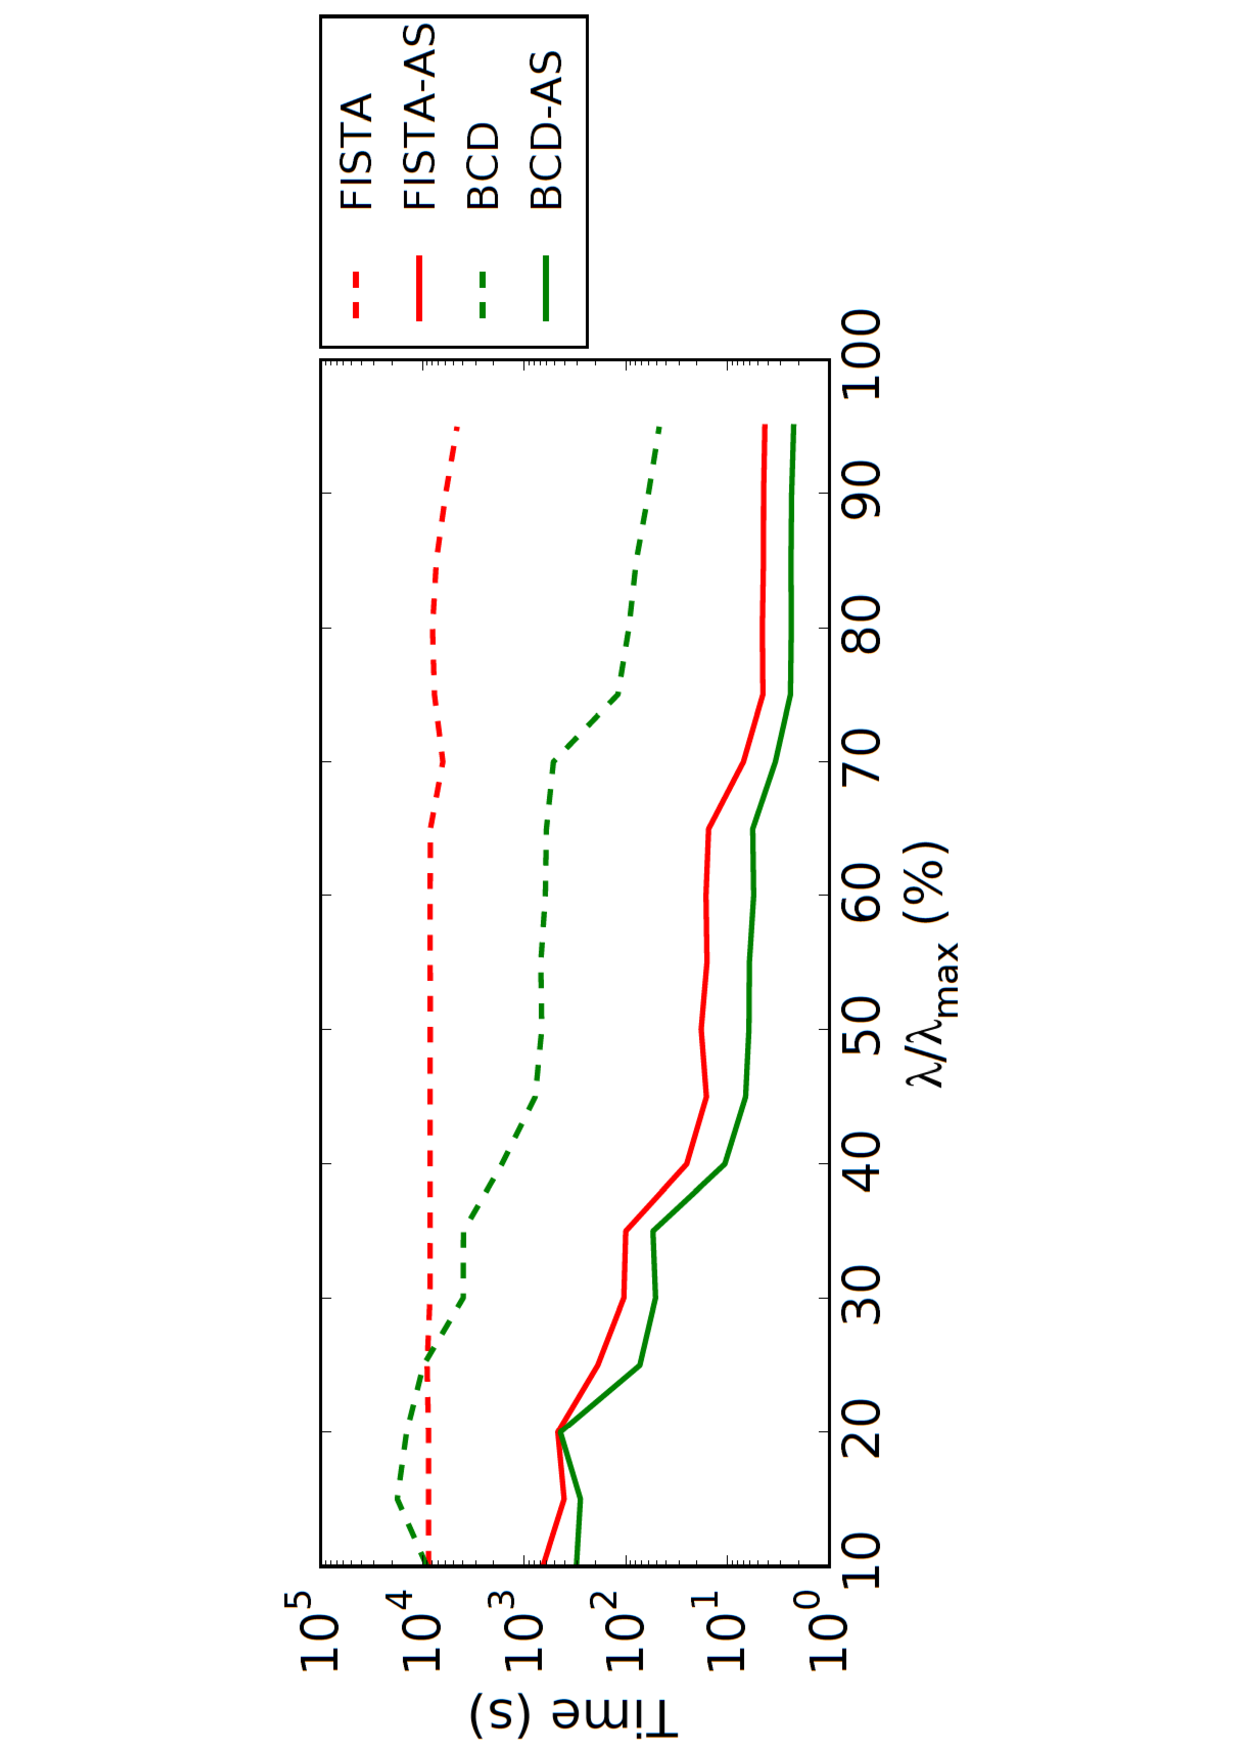
\includegraphics[trim={1cm 0.5cm 2cm 0.5cm},angle=270,width=0.95\textwidth]{background/comparison_fista_bcd}
    \caption{Computation time as a function of $\lambda$ for group \ac{lasso} on real MEG data using BCD and FISTA with (solid) and without (dashed) active set strategy. The size of the data was: 306 sensors, 7498 cortical locations, and free orientation (O=3)}
    \label{fig:comparison_fista_bcd}
\end{figure}
%\textbf{XXX: need to say what is $\lambda_{max}$ somewhere in this chapter}
Combining the BCD and the active set strategy reduces the computation time by a factor of 100 and allows us to compute the group \ac{lasso} on real MEG/EEG data in a few seconds. All the experimental results shown in the rest of this thesis will be obtained by using BCD with active set strategy.

\subsection{Conclusion}
This chapter gives all the needed background which has been used to develop and demonstrate the upcoming results. It demonstrated how to model the inverse problem as a regularized regression problem. It defined the multiple priors that have been used in the literature including the sparse approaches that are of interest in this thesis. Then it introduced some of the methods for solving the different convex optimization problems. This is again not an exhaustive list and not all details have been presented here. 

This chapter also defined the state of the art of the MEG/EEG inverse problem and how research in this field have been evolving. From the penalized regression formulation to the hierarchical Bayesian formulation, I will show in the next chapters how this thesis tries to bridge the gap between those two communities. Especially, the aim is to take advantage of each part, the computationally fast solvers developed so far by one community and the ability to quantify uncertainties of the solution in the second community.